% 'draft' mode can be used to speed up compilation
\documentclass[twoside,final]{hcmut-report}
\usepackage{codespace}

% Encodings
\usepackage{gensymb,textcomp}

% Better tables
% Wide tables go to https://tex.stackexchange.com/q/332902
\usepackage{array,longtable,multicol,multirow,siunitx,tabularx}

% Better enum
\usepackage{enumitem}

% Graphics
\usepackage{caption,float}
\graphicspath{{./}{../outputs/figures/}}

% Add options for figures, like max width, framing, etc.
\usepackage[export]{adjustbox}

% References
% Use \Cref{} instead of \ref{}
\usepackage[nameinlink]{cleveref}

% Configurations
\coursename{Machine Learning}
\reporttype{Báo cáo Bài tập lớn}
\title{Tên đề tài báo cáo}
\advisor{& Giảng viên hướng dẫn &}
\stuname{%
  & Phạm Viết Trường & 2413749 \\
  & Tên B & MSSV \\
  & Tên C & MSSV \\
   & Tên D & MSSV \\
  % & SV & MSSV \\
}

% Set depth of numbering for counters
\AtBeginDocument{\counterwithin{lstlisting}{section}}

% Rename some sections (uncomment to switch to Vietnamese headings)
%\AtBeginDocument{\renewcommand*{\contentsname}{Mục lục}}
%\AtBeginDocument{\renewcommand*{\listfigurename}{Danh sách hình ảnh}}
%\AtBeginDocument{\renewcommand*{\listtablename}{Danh sách bảng}}
%\AtBeginDocument{\renewcommand*{\lstlistlistingname}{Danh sách đoạn mã}}
%\AtBeginDocument{\renewcommand*{\refname}{Tài liệu tham khảo}}
%\AtBeginDocument{\renewcommand*{\bibname}{Tài liệu tham khảo}}

\begin{document}
\coverpage%

%\section*{Danh sách thành viên \& Phân công}
%\newcounter{memberrowno}
%\setcounter{memberrowno}{0}
%\begin{center}
%  \begin{tabular}{>{\stepcounter{memberrowno}\thememberrowno}llcc}
%    \toprule
%    \multicolumn{1}{c}{\textbf{STT}} & \textbf{Họ và tên} & \textbf{MSSV} & \textbf{Đóng góp} \\
%    \midrule
%                                     & Tùng               & xxxxxxx       & 100\%             \\
%                                     & Thành viên B       & xxxxxxx       & 100\%             \\
%                                     & Thành viên C       & xxxxxxx       & 100\%             \\
%                                     & Hiền               & xxxxxxx       & 100\%             \\
%    \bottomrule
%  \end{tabular}
%\end{center}
%\clearpage

\tableofcontents
\listoffigures
\listoftables
\lstlistoflistings{}

\clearpage

% ==============================================================================
% 1. Giới thiệu bài toán
% ==============================================================================
\section{Giới thiệu bài toán}\label{sec:gioi-thieu}
\subsection{Giới thiệu vấn đề}\label{subsec:gioi-thieu-van-de}
Ngày nay, việc thanh toán đang ngày càng trở nên tiện lợi khi mà người dùng không cần sử dụng tiền mặt và sự triển của thương mại điện tử đang ngày càng thúc đẩy các giao dịch thông qua thẻ tín trở nên phổ biến hơn. Tuy nhiên, sự tiện lợi đó cũng đi kèm với nhiều rủi ro về lỗ hổng bảo mật, và các giao dịch có hành vi gian lận đang ngày càng trở nên tinh vi và khó phát hiện hơn. Những giao bất chính này không chỉ gây ra thiệt hại về mặt tài chính mà còn làm xói mòn niềm tin của những khách hàng đối với các hệ thống ngân hàng. 

Do đó, việc xây dựng một hệ thống tự động có khả năng phát hiện và ngăn chặn các giao dịch bất thường là việc vô cùng thiết thực và cần thiết đối với các doanh nghiệp trong lĩnh tài chính nói chung và ngân hàng nói riêng 

\subsection{Đặt vấn đề}\label{subsec:dat-van-de}
Bài toán phát hiện gian lận thẻ tín dụng là bài toán phân loại nhị phân dựa trên dữ liệu lịch sử giao dịch. Tuy nhiên, để giải quyết bài toán này cần phải đối mặt với ba thách thức:
\begin{itemize}
    \item \textbf{Sự mất cân bằng dữ liệu nghiêm trọng:} Trong thực tế, số lượng giao dịch gian lận chỉ chiếm tỷ lệ cực nhỏ ($0.17\%$) so với tổng các giao dịch hợp lệ. Sự mất cân bằng này khiến cho việc chọn metric đánh giá trở nên khó khăn khi mà các chỉ số như \textbf{Accurancy} hay \textbf{ROC} sẽ dễ gây hiểu lầm do bị chi phối bởi lớp đa số; do đó, bài toán cần ưu tiên các metric phù hợp hơn như \textbf{Precision}, \textbf{Recall}, \textbf{F1-score} hoặc \textbf{PR-AUC}
    \item \textbf{Trade-off giữa Precision và Recall:} Nếu mô hình bỏ sót giao dịch gian lận, ngân hàng sẽ phải gánh chịu các thiệt hại về tài chính. Ngược lại nếu mô hình dự đoán nhầm các giao dịch hợp lệ thành giao dịch gian lận, thẻ của khách hàng có thể sẽ bị khóa và gây gián đoạn giao dịch, ảnh hưởng tới trải nghiệm của khách hàng.
    \item \textbf{Tính bảo mật và ẩn danh dữ liệu:} Để bảo vệ quyền riêng tư của chủ thẻ, dữ liệu đầu vào sẽ được xử lý thông qua biến đổi PCA, từ đó khiến việc nhận diện và đánh giá ý nghĩa và vai trò của các feature gặp nhiều hạn chế do không biết ý nghĩa nghiệp vụ của đặc trưng đó là gì.
\end{itemize}

\subsection{Mục tiêu dự án}\label{subsec:muc-tieu-du-an}
Trong bài tập lớn này, nhóm sẽ tập trụng và các mục tiêu chính sau:
\begin{itemize}
    \item Tối ưu hóa khả năng phát hiện giao dịch gian lận bằng cách nâng cao chỉ số \textbf{Recall} và \textbf{PR-AUC} trong khi vân giữ \textbf{Precision} ở mức có thể chấp nhận.
    
\end{itemize}

% ==============================================================================
% 2. Tiền xử lý dữ liệu
% ==============================================================================
\clearpage
\section{Tiền xử lý dữ liệu}\label{sec:tien-xu-ly}
% Phụ trách: Tùng
% Nhiệm vụ: Tiền xử lý dữ liệu — Thực hiện EDA

\subsection{Khai phá dữ liệu}\label{subsec:eda}
\subsubsection*{Tổng quan dữ liệu}
Tập dữ liệu này bao gồm các giao dịch bằng thẻ tín dụng được thực hiện vào tháng 9 năm 2013 bởi các chủ thẻ tại châu Âu.
Tập dữ liệu ghi lại các giao dịch diễn ra trong hai ngày, trong đó có 492 giao dịch gian lận trên tổng số 284.807 giao dịch.

Tập dữ liệu bao gồm các biến đầu vào đã được xử lý bằng PCA. Vì lý do bảo mật nên thông tin của các đặc trưng gốc không được cung cấp. Các đặc trưng từ $V1, V2, …, V28$ là những thành phần chính thu được từ PCA; các đặc trưng duy nhất không trải qua biến đổi PCA là \textbf{Time} và \textbf{Amount}.

Trong đó:
\begin{itemize}
    \item \textbf{Time}: ghi lại số giây trôi qua giữa mỗi giao dịch và giao dịch đầu tiên trong tập dữ liệu (0: Giao dịch đầu tiên, 10: Giao dịch xảy ra 10 giây sau giao dịch đầu tiên, 100:  Giao dịch xảy ra 100 giây sau giao dịch đầu tiên)
    \item \textbf{Amount}: là số tiền của giao dịch.
\end{itemize}
  
Feature \textbf{Class} là biến mục tiêu nhị phân với $1$ phản ánh giao dịch gian lận và $0$ trong các trường hợp còn lại.

\begin{table}[htbp]
\centering
\caption{Tổng quan dữ liệu của tập dữ liệu gồm $284807$ dòng và $31$ cột}
    \begin{tabular}{|clcc|}
    \hline
    \textbf{STT} & \textbf{Đặc trưng} & \textbf{Missing value} & \textbf{Kiểu dữ liệu} \\ \hline
    0 & Time & 0 & float64 \\ \hline
    1 -- 28 & V1 -- 28 & 0 & float64 \\ \hline
    29 & Amount & 0 & float64 \\ \hline
    30 & Class & 0 & int64 \\ \hline
    \end{tabular}
\end{table}
% Phụ trách: Tùng
% Nhiệm vụ: Tiền xử lý dữ liệu — Xây dựng pipeline tiền xử lý

\subsection{Xây dựng pipeline tiền xử lý}\label{subsec:pipeline-tien-xu-ly}
% TODO (Tùng): Mô tả chi tiết các bước làm sạch và biến đổi đặc trưng (tham chiếu src/preprocess.py):
% - Loại bỏ dữ liệu trùng lặp.
% - Biến đổi Time thành các đặc trưng chu kỳ (Hour_sin, Hour_cos).
% - Biến đổi log1p cho Amount (Log_Amount) và chuẩn hóa (RobustScaler).
% - Quy trình đóng gói thành pipeline tránh data leakage.

\textit{[Nội dung mục Xây dựng pipeline tiền xử lý đang chờ hoàn thiện.]}


% ==============================================================================
% 3. Mô hình và phương pháp
% ==============================================================================
\clearpage
\section{Mô hình và phương pháp}\label{sec:mo-hinh-phuong-phap}

% \subsection{Nhóm mô hình Baseline}\label{subsec:baseline}
% Phụ trách: B + C
% Nhiệm vụ: Xây dựng baseline — Logistic Regression

\subsubsection{Logistic Regression}\label{subsubsec:logistic-regression}
% TODO (B + C): Trình bày cơ sở lý thuyết và cấu hình mô hình Logistic Regression:
% - Công thức hàm dự đoán (sigmoid), hàm mất mát (binary cross-entropy / log-loss) và regularization (L1/L2).
% - Thiết lập siêu tham số (C, penalty, class_weight, max_iter...) trong src/model_b.py hoặc src/model_c.py.

\textit{[Nội dung mục Logistic Regression đang chờ hoàn thiện.]}

\subsection{Artificial Neural Network (ANN -- MLP)}\label{subsec:ann}

\subsubsection{Cơ sở lý thuyết}

\paragraph{1. Kiến trúc mạng truyền thẳng nhiều tầng (Multi-Layer Perceptron)}\mbox{}\\
Xét tập dữ liệu huấn luyện gồm $N$ mẫu $\{(\mathbf{x}_n, y_n)\}_{n=1}^{N}$, trong đó $\mathbf{x}_n \in \mathbb{R}^D$ là vector đặc trưng đầu vào và nhãn nhị phân $y_n \in \{0, 1\}$ đại diện lần lượt cho hai lớp $\mathcal{C}_0$ (bình thường) và $\mathcal{C}_1$ (gian lận). Mạng nơ-ron nhân tạo truyền thẳng nhiều tầng (\textit{Multi-Layer Perceptron -- MLP}) là mô hình học có giám sát có khả năng xấp xỉ các ánh xạ phi tuyến phức tạp thông qua $L$ tầng kết nối đầy đủ (\textit{fully-connected layers}), bao gồm tầng đầu vào ($\mathbf{a}^{(0)} = \mathbf{x}$), các tầng ẩn ($l = 1, \dots, L - 1$) và tầng đầu ra ($l = L$).

Tại mỗi tầng $l \in \{1, \dots, L\}$, quá trình lan truyền xuôi (\textit{forward propagation}) thực hiện phép biến đổi tuyến tính theo sau bởi hàm kích hoạt phi tuyến $g^{(l)}(\cdot)$:
\begin{equation}
    \mathbf{z}^{(l)} = \mathbf{W}^{(l)} \mathbf{a}^{(l-1)} + \mathbf{b}^{(l)}, \qquad \mathbf{a}^{(l)} = g^{(l)}\big(\mathbf{z}^{(l)}\big)
\end{equation}
trong đó $\mathbf{W}^{(l)} \in \mathbb{R}^{d_l \times d_{l-1}}$ là ma trận trọng số kết nối giữa tầng $l - 1$ và tầng $l$, $\mathbf{b}^{(l)} \in \mathbb{R}^{d_l}$ là vector độ lệch (\textit{bias}), và $d_l$ là số nơ-ron tại tầng $l$. Kiến trúc mạng MLP với hai tầng ẩn được minh họa tại Hình~\ref{fig:ann-architecture}.

\begin{figure}[H]
    \centering
    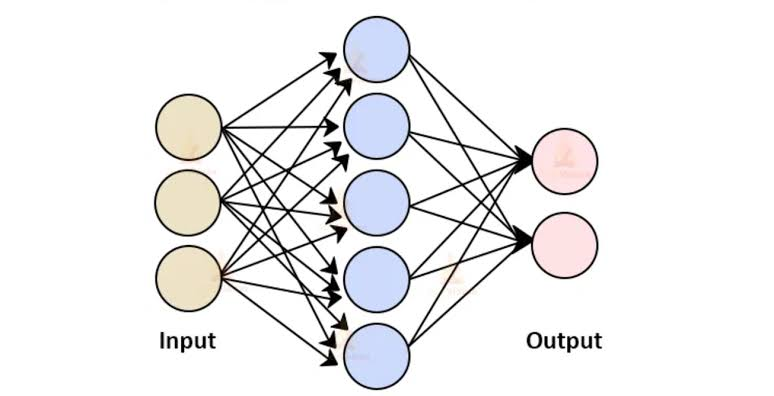
\includegraphics[width=0.75\linewidth]{graphics/ann_architecture.jpg}
    \caption{Minh họa kiến trúc mạng nơ-ron truyền thẳng nhiều tầng (MLP) với hai tầng ẩn}
    \label{fig:ann-architecture}
\end{figure}

\paragraph{2. Hàm kích hoạt phi tuyến (ReLU và Sigmoid)}\mbox{}\\
Nhằm tránh việc hợp thành nhiều tầng tuyến tính suy biến thành một ánh xạ tuyến tính duy nhất, các tầng ẩn sử dụng hàm kích hoạt \textbf{ReLU} (\textit{Rectified Linear Unit}):
\begin{equation}
    g_{\text{ReLU}}(z) = \max(0, z), \qquad g'_{\text{ReLU}}(z) = \begin{cases}
        1 & \text{nếu } z > 0 \\
        0 & \text{nếu } z \le 0
    \end{cases}
\end{equation}
Hàm ReLU giúp tính toán nhanh, tạo biểu diễn thưa cho các nơ-ron ẩn và giảm đáng kể hiện tượng triệt tiêu đạo hàm (\textit{vanishing gradient}) trên miền dương so với Sigmoid hoặc Tanh (Hình~\ref{fig:ann-relu}).

\begin{figure}[H]
    \centering
    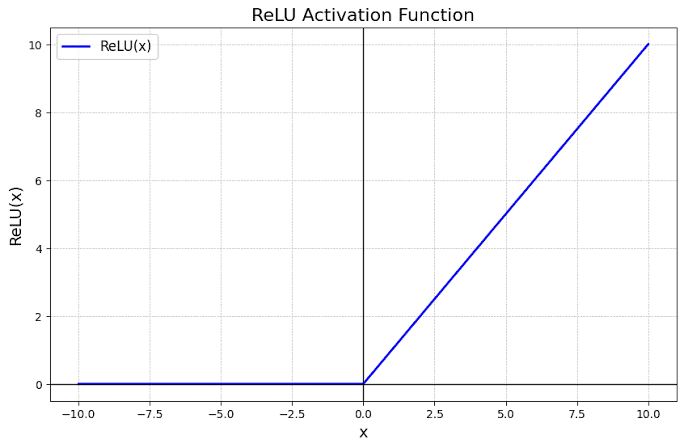
\includegraphics[width=0.65\linewidth]{graphics/ann_relu.png}
    \caption{Đồ thị hàm kích hoạt ReLU $g(z) = \max(0, z)$ và đạo hàm $g'(z)$}
    \label{fig:ann-relu}
\end{figure}

Tại tầng đầu ra ($l = L$, $d_L = 1$), đầu ra tuyến tính $z^{(L)}$ đi qua hàm kích hoạt \textbf{Sigmoid} để ước lượng xác suất hậu nghiệm thuộc lớp gian lận $\mathcal{C}_1$:
\begin{equation}
    \hat{y} \triangleq p(\mathcal{C}_1 \mid \mathbf{x}, \Theta) = \sigma\big(z^{(L)}\big) = \frac{1}{1 + e^{-z^{(L)}}} \in (0, 1)
\end{equation}
với $\Theta = \{(\mathbf{W}^{(l)}, \mathbf{b}^{(l)})\}_{l=1}^{L}$ là tập toàn bộ tham số cần học. Nhãn dự đoán $\hat{t} \in \{0, 1\}$ được xác định theo ngưỡng quyết định $\lambda$ (mặc định $\lambda = 0.5$): $\hat{t} = 1$ nếu $\hat{y} \ge \lambda$ và $\hat{t} = 0$ nếu ngược lại.

\paragraph{3. Hàm mất mát, Lan truyền ngược và Bộ tối ưu Adam}\mbox{}\\
Để huấn luyện mô hình phân loại nhị phân đồng thời kiểm soát độ phức tạp trọng số chống quá khớp (\textit{overfitting}), hàm mục tiêu sử dụng \textbf{Binary Cross-Entropy} kết hợp thành phần điều chuẩn \textbf{L2} (\textit{weight decay}):
\begin{equation}
    \mathcal{J}(\Theta) = -\frac{1}{N} \sum_{n=1}^{N} \left[ y_n \log \hat{y}_n + (1 - y_n) \log(1 - \hat{y}_n) \right] + \frac{\alpha}{2N} \sum_{l=1}^{L} \|\mathbf{W}^{(l)}\|_F^2
\end{equation}
trong đó $\alpha > 0$ là hệ số điều chuẩn L2 và $\|\cdot\|_F$ là chuẩn Frobenius của ma trận trọng số.

Gradient của hàm mục tiêu $\mathbf{g}_t = \nabla_{\Theta}\mathcal{J}(\Theta_{t-1})$ trên từng \textit{mini-batch} được tính hiệu quả bằng thuật toán \textbf{lan truyền ngược (Backpropagation)} dựa trên quy tắc dây chuyền (\textit{chain rule}). Quá trình cập nhật tham số sử dụng bộ tối ưu \textbf{Adam} (\textit{Adaptive Moment Estimation}), kết hợp ước lượng trung bình trượt hàm mũ của gradient bậc nhất ($\mathbf{m}_t$) và bình phương gradient bậc hai ($\mathbf{v}_t$):
\begin{equation}
    \mathbf{m}_t = \beta_1 \mathbf{m}_{t-1} + (1 - \beta_1)\mathbf{g}_t, \qquad \mathbf{v}_t = \beta_2 \mathbf{v}_{t-1} + (1 - \beta_2)\mathbf{g}_t^2
\end{equation}
Sau khi hiệu chỉnh độ chệch khởi tạo $\hat{\mathbf{m}}_t = \frac{\mathbf{m}_t}{1 - \beta_1^t}$ và $\hat{\mathbf{v}}_t = \frac{\mathbf{v}_t}{1 - \beta_2^t}$, tham số mạng được cập nhật theo công thức:
\begin{equation}
    \Theta_t = \Theta_{t-1} - \eta \frac{\hat{\mathbf{m}}_t}{\sqrt{\hat{\mathbf{v}}_t} + \epsilon}
\end{equation}
trong đó $\eta$ là tốc độ học ban đầu, $\beta_1, \beta_2 \in [0, 1)$ là các hệ số suy giảm mô-men và $\epsilon > 0$ giúp ổn định số học khi chia. Nhờ cơ chế tự điều chỉnh tốc độ học riêng cho từng tham số, Adam hội tụ nhanh và ổn định trên dữ liệu quy mô lớn.

\subsubsection{Áp dụng mô hình vào bài toán}

\paragraph{1. Môi trường và Thư viện sử dụng}\mbox{}\\
Mô hình được cài đặt bằng ngôn ngữ \textbf{Python} với hai thư viện chính:
\begin{itemize}
    \item \texttt{scikit-learn}: Cung cấp lớp \texttt{MLPClassifier} để xây dựng và huấn luyện mạng nơ-ron nhiều tầng, cùng \texttt{RobustScaler} và \texttt{StratifiedKFold} cho bước chuẩn hóa và kiểm định chéo.
    \item \texttt{NumPy}: Hỗ trợ xử lý mảng và tính toán vector hóa dữ liệu.
\end{itemize}

\paragraph{2. Quy trình tiền xử lý và Huấn luyện}\mbox{}\\
Quy trình thực nghiệm trong tệp \texttt{src/model\_ANN.py} tuân thủ chặt chẽ nguyên tắc cô lập tập kiểm định để tránh rò rỉ dữ liệu (\textit{data leakage}):
\begin{enumerate}
    \item \textbf{Phân chia dữ liệu phân tầng:} Tập dữ liệu sau làm sạch được tách thành tập huấn luyện toàn phần và tập kiểm tra độc lập (\texttt{split\_train\_test}), kết hợp kiểm định chéo \textit{Stratified K-Fold} nhằm giữ nguyên tỷ lệ lớp gian lận trên từng \textit{fold}.
    \item \textbf{Chuẩn hóa đặc trưng kháng ngoại lai:} Do mạng nơ-ron tối ưu theo gradient nên rất nhạy với độ lớn đầu vào. Trong khi các thành phần \texttt{V1--V28} đã qua biến đổi PCA, cột đặc trưng giao dịch (\texttt{COLS\_TO\_SCALE}) được chuẩn hóa bằng \texttt{RobustScaler} (chỉ \texttt{fit\_transform} trên tập huấn luyện con rồi \texttt{transform} sang tập kiểm định).
    \item \textbf{Huấn luyện có dừng sớm và Đánh giá:} Trong từng \textit{fold}, mô hình \texttt{MLPClassifier} được huấn luyện với cơ chế \texttt{early\_stopping=True} (tự động trích $10\%$ tập huấn luyện làm tập kiểm định nội bộ để dừng sớm khi hiệu năng không cải thiện, vừa hạn chế quá khớp vừa rút ngắn thời gian chạy). Sau khi hoàn tất kiểm định chéo, mô hình cuối cùng được huấn luyện lại trên toàn bộ tập huấn luyện đã chuẩn hóa và đánh giá trên tập kiểm tra với ngưỡng phân loại $\lambda = 0.5$ qua mô-đun \texttt{src/metrics.py}.
\end{enumerate}

\paragraph{3. Thiết lập siêu tham số}\mbox{}\\
Cấu hình chi tiết trong hàm \texttt{build\_model()} của tệp \texttt{src/model\_ANN.py} được tổng hợp tại Bảng~\ref{tab:ann_hyperparams}.

\begin{table}[H]
\centering
\caption{Thiết lập siêu tham số cho mô hình Artificial Neural Network (\texttt{src/model\_ANN.py})}
\label{tab:ann_hyperparams}
\renewcommand{\arraystretch}{1.2}
\begin{tabular}{|l|l|p{8.0cm}|}
\hline
\textbf{Siêu tham số} & \textbf{Giá trị} & \textbf{Mục đích sử dụng} \\
\hline
\texttt{hidden\_layer\_sizes} & \texttt{(64, 32)} & Thiết kế 2 tầng ẩn với 64 và 32 nơ-ron, đủ khả năng biểu diễn quan hệ phi tuyến mà vẫn gọn nhẹ, tránh quá khớp. \\
\hline
\texttt{activation} & \texttt{"relu"} & Hàm kích hoạt ReLU cho các tầng ẩn, tăng tốc độ tính toán và hạn chế triệt tiêu gradient. \\
\hline
\texttt{solver} & \texttt{"adam"} & Bộ tối ưu hóa Adam thích ứng tốc độ học theo từng tham số, hội tụ nhanh trên dữ liệu lớn. \\
\hline
\texttt{max\_iter} & \texttt{50} & Giới hạn tối đa 50 vòng lặp (\textit{epochs}) giúp kiểm soát thời gian huấn luyện trên toàn bộ 5 \textit{folds}. \\
\hline
\texttt{early\_stopping} & \texttt{True} & Tự động dừng sớm dựa trên tập kiểm định nội bộ ($10\%$) khi điểm số không còn cải thiện, hạn chế quá khớp. \\
\hline
\texttt{random\_state} & \texttt{42} & Cố định hạt giống khởi tạo trọng số ngẫu nhiên và chia lô nhằm đảm bảo tính tái lập kết quả. \\
\hline
\end{tabular}
\end{table}

% Optional baseline (comment dòng dưới nếu không sử dụng):
% Phụ trách: B + C
% Nhiệm vụ: Xây dựng baseline — (Optional) SVM or Naive Bayes

\subsection{SVM}\label{subsubsec:svm-naive-bayes}

\subsubsection{Cơ sở lý thuyết}

\paragraph{1. Siêu phẳng phân tách và Bộ phân lớp lề cực đại}\mbox{}\\
Xét tập dữ liệu huấn luyện gồm $N$ mẫu $\{(\mathbf{x}_n, t_n)\}_{n=1}^{N}$, trong đó $\mathbf{x}_n \in \mathbb{R}^D$ là vector đặc trưng đầu vào và nhãn nhị phân $t_n \in \{-1, +1\}$ đại diện lần lượt cho hai lớp $\mathcal{C}_0$ (bình thường) và $\mathcal{C}_1$ (gian lận). Thông qua ánh xạ đặc trưng $\phi(\cdot)$ sang không gian nhiều chiều hơn, SVM tìm một siêu phẳng phân tách tuyến tính $y(\mathbf{x}) = \mathbf{w}^T \phi(\mathbf{x}) + b = 0$ sao cho khoảng cách từ siêu phẳng tới các điểm dữ liệu gần nhất của hai lớp (gọi là \textit{lề} -- margin, có độ rộng $\frac{2}{\|\mathbf{w}\|}$) đạt giá trị lớn nhất nhằm tối ưu khả năng tổng quát hóa (Hình~\ref{fig:svm-max-margin}).

\begin{figure}[H]
    \centering
    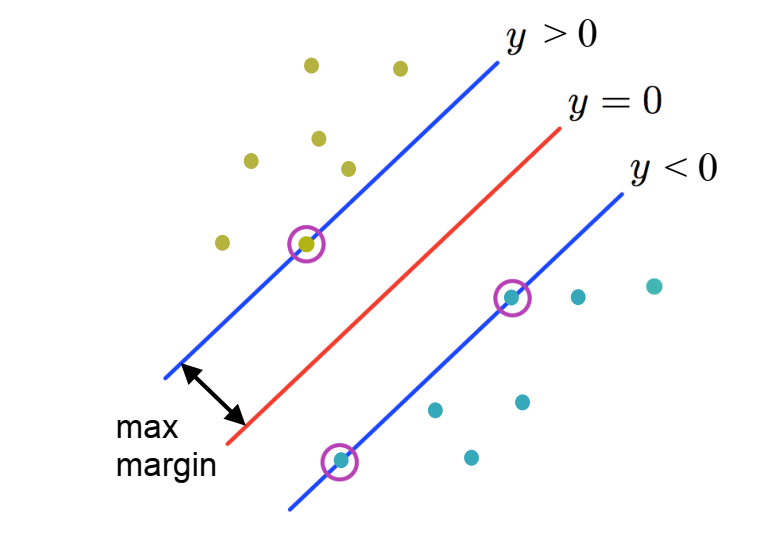
\includegraphics[width=0.72\linewidth]{graphics/svm_max_margin.png}
    \caption{Minh họa siêu phẳng phân tách lề cực đại và các vector hỗ trợ}
    \label{fig:svm-max-margin}
\end{figure}

\paragraph{2. SVM lề mềm và Bài toán đối ngẫu Lagrange}\mbox{}\\
Với dữ liệu thực tế có nhiễu và chồng lấp giữa hai lớp, mô hình bổ sung các biến bù $\xi_n \ge 0$ để cho phép một số điểm vi phạm ranh giới lề như minh họa tại Hình~\ref{fig:svm-soft-margin}. Bài toán tối ưu gốc của Soft-Margin SVM được phát biểu như sau:
\begin{equation}
    \min_{\mathbf{w}, b, \boldsymbol{\xi}} \; \frac{1}{2}\|\mathbf{w}\|^2 + C \sum_{n=1}^{N} \xi_n \qquad \text{với ràng buộc } \begin{cases} t_n\left(\mathbf{w}^T \phi(\mathbf{x}_n) + b\right) \ge 1 - \xi_n \\ \xi_n \ge 0 \end{cases}, \; \forall n = 1, \dots, N
\end{equation}
trong đó $C > 0$ là tham số điều chuẩn kiểm soát sự đánh đổi giữa việc mở rộng lề và mức phạt các điểm vi phạm.

\begin{figure}[H]
    \centering
    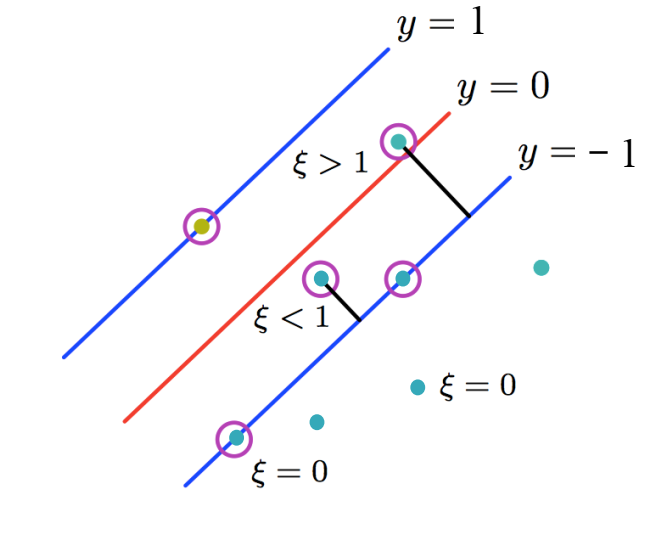
\includegraphics[width=0.72\linewidth]{graphics/svm_soft_margin.png}
    \caption{Cơ chế Soft-Margin SVM với các trường hợp giá trị của biến bù $\xi_n$}
    \label{fig:svm-soft-margin}
\end{figure}

Sử dụng nhân tử Lagrange $a_n \ge 0$, bài toán được chuyển sang dạng đối ngẫu:
\begin{equation}
    \max_{\mathbf{a}} \; \tilde{L}(\mathbf{a}) = \sum_{n=1}^{N} a_n - \frac{1}{2} \sum_{n=1}^{N} \sum_{m=1}^{N} a_n a_m t_n t_m K(\mathbf{x}_n, \mathbf{x}_m)
\end{equation}
thỏa mãn $0 \le a_n \le C$ và $\sum_{n=1}^{N} a_n t_n = 0$. Nhờ tính chất thưa (\textit{sparsity}), chỉ các điểm nằm trên hoặc vi phạm biên lề mới có $a_n > 0$ và được gọi là các \textbf{vector hỗ trợ} (tập $\mathcal{S}$), các điểm còn lại đều có $a_n = 0$. Hàm quyết định phân lớp khi đó chỉ phụ thuộc vào tập $\mathcal{S}$:
\begin{equation}
    y(\mathbf{x}) = \sum_{n \in \mathcal{S}} a_n t_n K(\mathbf{x}_n, \mathbf{x}) + b, \qquad \hat{t} = \text{sign}\big(y(\mathbf{x})\big)
\end{equation}

\paragraph{3. Kernel Trick và Hạt nhân RBF}\mbox{}\\
Thay vì tính tường minh tọa độ $\phi(\mathbf{x})$ trong không gian số chiều lớn (Hình~\ref{fig:svm-kernel-trick}), thủ thuật hạt nhân tính trực tiếp tích vô hướng thông qua hàm hạt nhân $K(\mathbf{x}_n, \mathbf{x}_m) = \phi(\mathbf{x}_n)^T \phi(\mathbf{x}_m)$. Với hạt nhân \textbf{RBF (Radial Basis Function / Gaussian)}, mức độ tương đồng giữa hai điểm dữ liệu được đo bằng khoảng cách Euclid:
\begin{equation}
    K_{\text{rbf}}(\mathbf{x}_n, \mathbf{x}_m) = \exp\left(-\gamma \|\mathbf{x}_n - \mathbf{x}_m\|^2\right)
\end{equation}
trong đó $\gamma > 0$ điều khiển độ rộng của phân phối Gaussian, kết hợp cùng tham số $C$ để định hình độ phức tạp của ranh giới quyết định phi tuyến (Hình~\ref{fig:svm-rbf-params}).

\begin{figure}[H]
    \centering
    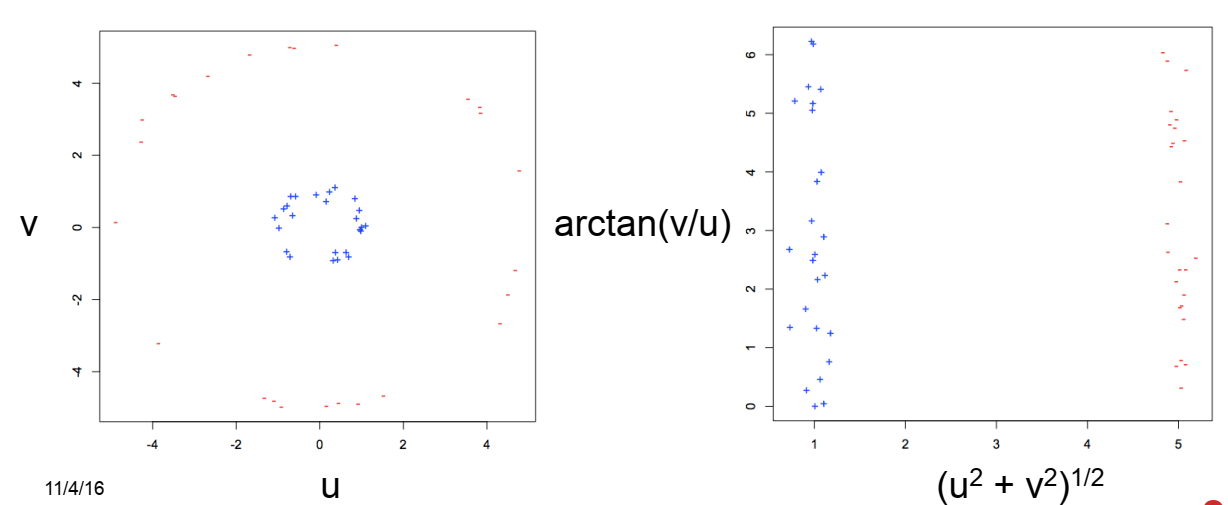
\includegraphics[width=0.82\linewidth]{graphics/svm_kernel_mapping.png}
    \caption{Ánh xạ dữ liệu không tách tuyến tính từ không gian gốc sang không gian đặc trưng chiều cao qua hàm $\phi(\mathbf{x})$}
    \label{fig:svm-kernel-trick}
\end{figure}

\begin{figure}[H]
    \centering
    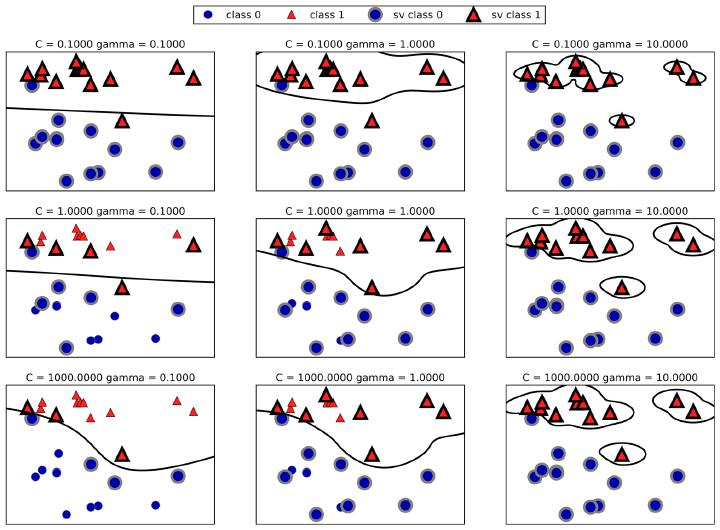
\includegraphics[width=0.85\linewidth]{graphics/svm_rbf_params.png}
    \caption{Ảnh hưởng của tham số điều chuẩn $C$ và độ rộng hạt nhân $\gamma$ lên ranh giới quyết định của RBF SVM}
    \label{fig:svm-rbf-params}
\end{figure}

\paragraph{4. Hiệu chỉnh xác suất hậu nghiệm (Platt Scaling)}\mbox{}\\
Do SVM thuần túy chỉ xuất giá trị khoảng cách có dấu $y(\mathbf{x})$ thay vì xác suất trực tiếp, kỹ thuật \textbf{Platt Scaling} được áp dụng bằng cách khớp một hàm Sigmoid lên đầu ra $y(\mathbf{x})$ thông qua kiểm định chéo nội bộ để ước lượng xác suất hậu nghiệm thuộc lớp gian lận $\mathcal{C}_1$:
\begin{equation}
    \hat{y} \triangleq p(\mathcal{C}_1 \mid \mathbf{x}) = \frac{1}{1 + \exp\big(A \, y(\mathbf{x}) + B\big)}
\end{equation}
với hai tham số vô hướng $A, B \in \mathbb{R}$ được tối ưu theo nguyên lý hợp lý cực đại trên các dự đoán ngoài \textit{fold}.

\subsubsection{Áp dụng mô hình vào bài toán}

\paragraph{1. Môi trường và Thư viện sử dụng}\mbox{}\\
Mô hình được triển khai bằng ngôn ngữ \textbf{Python} với các thư viện chính:
\begin{itemize}
    \item \texttt{scikit-learn}: Cung cấp bộ phân lớp \texttt{SVC}, \texttt{CalibratedClassifierCV} để hiệu chỉnh xác suất, \texttt{Pipeline} đóng gói luồng xử lý cùng hai bộ chuẩn hóa \texttt{RobustScaler} và \texttt{StandardScaler}.
    \item \texttt{imbalanced-learn}: Cung cấp kỹ thuật giảm mẫu ngẫu nhiên \texttt{RandomUnderSampler}.
    \item \texttt{NumPy}: Xử lý mảng và tính toán vector hóa.
\end{itemize}

\paragraph{2. Quy trình tiền xử lý, Cân bằng dữ liệu và Huấn luyện}\mbox{}\\
Quy trình thực nghiệm trong tệp \texttt{src/model\_b\_2.py} được thiết kế chặt chẽ nhằm ngăn ngừa rò rỉ dữ liệu (\textit{data leakage}) và tối ưu hóa độ phức tạp tính toán của Kernel SVM:
\begin{enumerate}
    \item \textbf{Chia dữ liệu phân tầng:} Dữ liệu sau làm sạch được tách thành tập huấn luyện toàn phần và tập kiểm tra độc lập, kết hợp kiểm định chéo \textit{Stratified K-Fold} để duy trì tỷ lệ lớp gian lận trên từng \textit{fold}.
    \item \textbf{Chuẩn hóa dữ liệu hai bước:} Do hạt nhân RBF dựa trên khoảng cách Euclid $\|\mathbf{x}_n - \mathbf{x}_m\|^2$ nên rất nhạy với chênh lệch thang đo giữa các chiều đặc trưng. Trong từng \textit{fold}, các cột số (\texttt{COLS\_TO\_SCALE}) trước tiên được chuẩn hóa bằng \texttt{RobustScaler} để triệt tiêu ảnh hưởng của ngoại lai, sau đó toàn bộ đặc trưng đi qua \texttt{StandardScaler} ($x'' = \frac{x' - \mu}{\sigma}$) bên trong \texttt{Pipeline} để đưa về trung bình $0$ và phương sai đơn vị.
    \item \textbf{Giảm mẫu lớp đa số trên tập huấn luyện:} Vì độ phức tạp huấn luyện của Kernel SVM tăng theo cấp số nhân với số lượng mẫu ($O(N^2)$ đến $O(N^3)$), kỹ thuật \texttt{RandomUnderSampler} với \texttt{sampling\_strategy=0.05} được áp dụng riêng trên tập huấn luyện con. Bước này giữ nguyên $100\%$ mẫu gian lận ($\mathcal{C}_1$) và lấy mẫu ngẫu nhiên lớp bình thường ($\mathcal{C}_0$) theo tỷ lệ $20:1$, trong khi tập kiểm định và tập kiểm tra giữ nguyên phân phối thực tế.
    \item \textbf{Hiệu chỉnh xác suất và Đánh giá:} Mô hình \texttt{SVC} được bọc trong \texttt{CalibratedClassifierCV} (\texttt{cv=5}, \texttt{method="sigmoid"}) để xuất xác suất dự đoán trên tập kiểm tra với ngưỡng phân loại $\lambda = 0.5$ và đánh giá qua mô-đun \texttt{src/metric\_model\_b\_2.py}.
\end{enumerate}

\paragraph{3. Thiết lập siêu tham số}\mbox{}\\
Cấu hình các siêu tham số cốt lõi trong hàm \texttt{handle\_imbalance()} và \texttt{build\_model()} được tổng hợp tại Bảng~\ref{tab:svm_hyperparams}.

\begin{table}[H]
\centering
\caption{Thiết lập siêu tham số cho mô hình Kernel SVM (\texttt{src/model\_b\_2.py})}
\label{tab:svm_hyperparams}
\renewcommand{\arraystretch}{1.2}
\begin{tabular}{|l|l|p{8.0cm}|}
\hline
\textbf{Thành phần / Tham số} & \textbf{Giá trị} & \textbf{Mục đích sử dụng} \\
\hline
\texttt{sampling\_strategy} & \texttt{0.05} & Giữ toàn bộ lớp gian lận và giảm mẫu lớp bình thường về tỷ lệ $20:1$, giảm chi phí tính toán và hạn chế thiên lệch. \\
\hline
\texttt{kernel} & \texttt{"rbf"} & Sử dụng hạt nhân Gaussian RBF để ánh xạ dữ liệu sang không gian phi tuyến chiều cao. \\
\hline
\texttt{C} & \texttt{2.0} & Tham số phạt biến bù của Soft-Margin SVM, tăng nhẹ độ chặt của ranh giới phân tách so với mặc định. \\
\hline
\texttt{gamma} & \texttt{"scale"} & Tự động tính $\gamma = \frac{1}{D \cdot \text{Var}(\mathbf{X})}$, điều chỉnh độ rộng hạt nhân thích ứng với phương sai dữ liệu. \\
\hline
\texttt{CalibratedClassifierCV} & \texttt{cv=5, sigmoid} & Thực hiện Platt Scaling qua kiểm định chéo 5-fold (\texttt{ensemble=False}) để hiệu chỉnh đầu ra thành xác suất tin cậy. \\
\hline
\texttt{random\_state} & \texttt{RANDOM\_STATE} & Cố định hạt giống ngẫu nhiên cho cả bộ giảm mẫu và mô hình SVC nhằm đảm bảo tính tái lập. \\
\hline
\end{tabular}
\end{table}

% Optional advanced models (comment mục dưới nếu không sử dụng):
% \subsection{Nhóm mô hình nâng cao (Optional)}\label{subsec:mo-hinh-nang-cao}
\subsection{Ensemble Learning -- XGBoost}\label{subsec:ensemble-learning}

\subsubsection{Cơ sở lý thuyết}

\paragraph{1. Nguyên lý học tổ hợp và Mô hình cộng dồn Gradient Boosting}\mbox{}\\
Học tổ hợp (\textit{Ensemble Learning}) là phương pháp kết hợp nhiều mô hình cơ sở (\textit{weak learners}) nhằm tạo ra một bộ dự đoán mạnh hơn và ổn định hơn từng mô hình đơn lẻ. Hai chiến lược phổ biến là \textit{Bagging} (huấn luyện song song nhiều mô hình độc lập để giảm phương sai) và \textit{Boosting} (huấn luyện tuần tự sao cho mỗi mô hình mới tập trung sửa sai cho các mô hình trước đó để giảm độ chệch).

\textbf{XGBoost} (\textit{eXtreme Gradient Boosting}) là biến thể tối ưu hiệu năng cao của thuật toán Gradient Boosted Decision Trees (GBDT). Với tập dữ liệu $N$ mẫu $\{(\mathbf{x}_n, y_n)\}_{n=1}^{N}$ ($\mathbf{x}_n \in \mathbb{R}^D$, $y_n \in \{0, 1\}$), XGBoost biểu diễn điểm dự đoán thô $\hat{z}_n$ dưới dạng tổng cộng dồn của $K$ cây quyết định hồi quy (CART):
\begin{equation}
    \hat{z}_n = \sum_{k=1}^{K} f_k(\mathbf{x}_n), \qquad f_k \in \mathcal{F}
\end{equation}
trong đó $\mathcal{F} = \{f(\mathbf{x}) = w_{q(\mathbf{x})}\}$ là không gian các cây hồi quy, $q(\mathbf{x}) \in \{1, \dots, T\}$ ánh xạ mẫu $\mathbf{x}$ tới chỉ số nút lá tương ứng và $w_j \in \mathbb{R}$ là trọng số của lá $j$. Đối với bài toán phân loại nhị phân, xác suất hậu nghiệm thuộc lớp gian lận $\mathcal{C}_1$ được suy ra qua hàm Sigmoid:
\begin{equation}
    \hat{y}_n \triangleq p(\mathcal{C}_1 \mid \mathbf{x}_n) = \sigma(\hat{z}_n) = \frac{1}{1 + e^{-\hat{z}_n}} \in (0, 1)
\end{equation}
Cơ chế xây dựng cây tuần tự của Gradient Boosting / XGBoost được minh họa tại Hình~\ref{fig:xgboost-boosting}.

\begin{figure}[H]
    \centering
    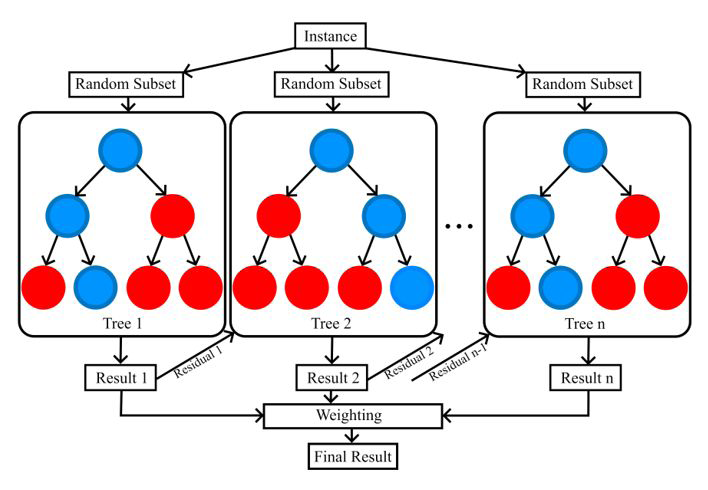
\includegraphics[width=0.80\linewidth]{graphics/xgboost_boosting.png}
    \caption{Minh họa cơ chế xây dựng tuần tự các cây quyết định trong mô hình XGBoost}
    \label{fig:xgboost-boosting}
\end{figure}

\paragraph{2. Hàm mục tiêu có điều chuẩn và Xấp xỉ Taylor bậc hai}\mbox{}\\
Điểm khác biệt cốt lõi giúp XGBoost vượt trội so với Gradient Boosting truyền thống là tích hợp trực tiếp thành phần điều chuẩn độ phức tạp cây $\Omega(f)$ vào hàm mục tiêu. Tại bước lặp thứ $t$, cây mới $f_t$ được bổ sung để cực tiểu hóa:
\begin{equation}
    \mathcal{L}^{(t)} = \sum_{n=1}^{N} l\!\left(y_n, \hat{z}_n^{(t-1)} + f_t(\mathbf{x}_n)\right) + \Omega(f_t), \qquad \Omega(f) = \gamma T + \frac{1}{2}\lambda_{\text{reg}} \sum_{j=1}^{T} w_j^2
\end{equation}
trong đó $l(y_n, \hat{z}_n) = -\left[y_n \log\sigma(\hat{z}_n) + (1 - y_n)\log(1 - \sigma(\hat{z}_n))\right]$ là hàm mất mát Binary Cross-Entropy, $T$ là số nút lá, $\gamma \ge 0$ phạt việc tạo thêm nút lá mới và $\lambda_{\text{reg}} \ge 0$ là hệ số điều chuẩn L2 giúp làm mượt trọng số lá, chống quá khớp.

Áp dụng khai triển Taylor bậc hai quanh $\hat{z}_n^{(t-1)}$ và loại bỏ các hằng số không phụ thuộc vào $f_t$, hàm mục tiêu xấp xỉ thu được có dạng:
\begin{equation}
    \tilde{\mathcal{L}}^{(t)} = \sum_{j=1}^{T} \left[ \left(\sum_{n \in I_j} g_n\right) w_j + \frac{1}{2}\left(\sum_{n \in I_j} h_n + \lambda_{\text{reg}}\right) w_j^2 \right] + \gamma T
\end{equation}
trong đó $I_j = \{n \mid q(\mathbf{x}_n) = j\}$ là tập các mẫu rơi vào nút lá $j$, còn $g_n$ và $h_n$ lần lượt là đạo hàm bậc nhất và bậc hai của hàm mất mát theo $\hat{z}_n^{(t-1)}$:
\begin{equation}
    g_n = \frac{\partial l(y_n, \hat{z}_n^{(t-1)})}{\partial \hat{z}_n^{(t-1)}} = \hat{y}_n^{(t-1)} - y_n, \qquad h_n = \frac{\partial^2 l(y_n, \hat{z}_n^{(t-1)})}{\partial (\hat{z}_n^{(t-1)})^2} = \hat{y}_n^{(t-1)}\big(1 - \hat{y}_n^{(t-1)}\big)
\end{equation}

\paragraph{3. Trọng số lá tối ưu, Tiêu chí chia nhánh (Gain) và Thuật toán Histogram}\mbox{}\\
Đặt $G_j = \sum_{n \in I_j} g_n$ và $H_j = \sum_{n \in I_j} h_n$. Với một cấu trúc cây cố định, nghiệm tối ưu của trọng số lá $w_j^*$ và giá trị hàm mục tiêu tương ứng đạt được bằng cách cho đạo hàm theo $w_j$ bằng $0$:
\begin{equation}
    w_j^* = -\frac{G_j}{H_j + \lambda_{\text{reg}}}, \qquad \tilde{\mathcal{L}}^{(t)*}(q) = -\frac{1}{2}\sum_{j=1}^{T} \frac{G_j^2}{H_j + \lambda_{\text{reg}}} + \gamma T
\end{equation}
Khi xét tách một nút thành hai nhánh trái ($I_L$) và phải ($I_R$), độ giảm mất mát (\textit{Gain}) được tính bằng:
\begin{equation}
    \text{Gain} = \frac{1}{2}\left[\frac{G_L^2}{H_L + \lambda_{\text{reg}}} + \frac{G_R^2}{H_R + \lambda_{\text{reg}}} - \frac{(G_L + G_R)^2}{H_L + H_R + \lambda_{\text{reg}}}\right] - \gamma
\end{equation}
Phép chia nhánh chỉ được chấp nhận khi $\text{Gain} > 0$. Sau khi xây dựng xong cây $f_t$, đóng góp của cây được nhân với tốc độ học $\eta \in (0, 1]$ (\textit{shrinkage}): $\hat{z}_n^{(t)} = \hat{z}_n^{(t-1)} + \eta f_t(\mathbf{x}_n)$ nhằm chừa không gian cho các cây sau tinh chỉnh dần và giảm nguy cơ quá khớp.

Nhằm tối ưu tốc độ trên dữ liệu bảng quy mô lớn, thuật toán chia nhánh theo biểu đồ tần suất (\texttt{tree\_method="hist"}) gom các giá trị đặc trưng liên tục vào các thùng rời rạc (\textit{bins}) và tích lũy tổng $(G, H)$ theo từng thùng (Hình~\ref{fig:xgboost-hist}), kết hợp tính toán song song trên nhiều lõi CPU giúp rút ngắn đáng kể thời gian huấn luyện mà vẫn duy trì độ chính xác cao.

\begin{figure}[H]
    \centering
    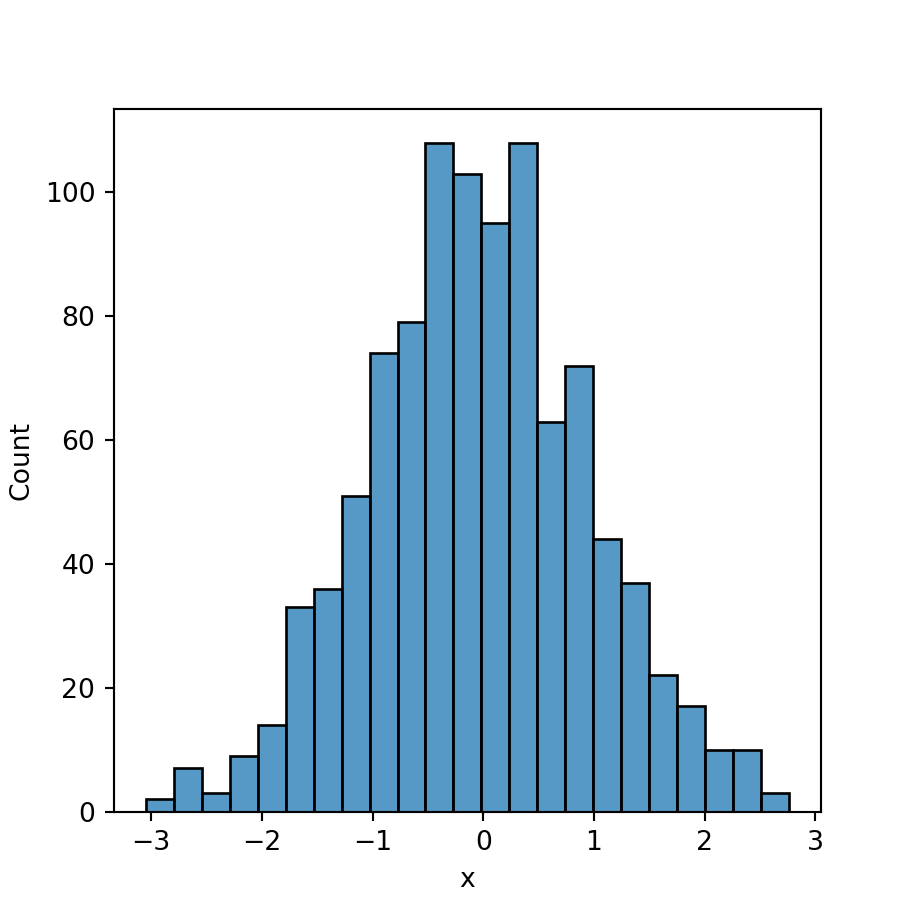
\includegraphics[width=0.78\linewidth]{graphics/xgboost_hist.png}
    \caption{Minh họa kỹ thuật rời rạc hóa đặc trưng theo thùng (\textit{histogram}) để tìm ngưỡng chia nhánh tối ưu trong XGBoost}
    \label{fig:xgboost-hist}
\end{figure}

\subsubsection{Áp dụng mô hình vào bài toán}

\paragraph{1. Môi trường và Thư viện sử dụng}\mbox{}\\
Mô hình được cài đặt bằng ngôn ngữ \textbf{Python} với các thư viện chính:
\begin{itemize}
    \item \texttt{xgboost}: Cung cấp lớp \texttt{XGBClassifier} để xây dựng và huấn luyện mô hình Gradient Boosted Trees hiệu năng cao.
    \item \texttt{scikit-learn}: Cung cấp \texttt{RobustScaler} cho bước chuẩn hóa đặc trưng và \texttt{StratifiedKFold} cho kiểm định chéo phân tầng.
    \item \texttt{NumPy}: Hỗ trợ tính toán mảng và xử lý vector hóa dữ liệu.
\end{itemize}

\paragraph{2. Quy trình tiền xử lý và Huấn luyện}\mbox{}\\
Quy trình thực nghiệm trong tệp \texttt{src/model\_ensemble.py} được đồng bộ với khung đánh giá chung của toàn hệ thống nhằm đảm bảo so sánh công bằng và không rò rỉ dữ liệu (\textit{data leakage}):
\begin{enumerate}
    \item \textbf{Phân chia dữ liệu phân tầng:} Dữ liệu sau tiền xử lý được chia thành tập huấn luyện toàn phần và tập kiểm tra độc lập, kết hợp kiểm định chéo \textit{Stratified K-Fold} để duy trì tỷ lệ giao dịch gian lận nhất quán qua từng \textit{fold}.
    \item \textbf{Chuẩn hóa đồng nhất theo từng fold:} Mặc dù mô hình dựa trên cây quyết định ít nhạy với biến đổi đơn điệu của đặc trưng, các cột thuộc \texttt{COLS\_TO\_SCALE} vẫn được chuẩn hóa bằng \texttt{RobustScaler} riêng biệt trong từng \textit{fold} (\texttt{fit\_transform} trên tập huấn luyện con, \texttt{transform} trên tập kiểm định) để đồng bộ hoàn toàn pipeline tiền xử lý với các mô hình khác.
    \item \textbf{Huấn luyện và Đánh giá:} Mô hình \texttt{XGBClassifier} giữ nguyên phân phối dữ liệu gốc (nhờ khả năng tách vùng phi tuyến mạnh của tổ hợp cây điều chuẩn), thực hiện đánh giá chéo trên 5 \textit{folds}, sau đó huấn luyện lại mô hình cuối cùng trên $100\%$ tập huấn luyện và đánh giá trên tập kiểm tra độc lập với ngưỡng phân loại $\lambda = 0.5$ thông qua mô-đun \texttt{src/metrics.py}.
\end{enumerate}

\paragraph{3. Thiết lập siêu tham số}\mbox{}\\
Cấu hình chi tiết trong hàm \texttt{build\_model()} của tệp \texttt{src/model\_ensemble.py} được tổng hợp tại Bảng~\ref{tab:xgb_hyperparams}.

\begin{table}[H]
\centering
\caption{Thiết lập siêu tham số cho mô hình XGBoost (\texttt{src/model\_ensemble.py})}
\label{tab:xgb_hyperparams}
\renewcommand{\arraystretch}{1.2}
\begin{tabular}{|l|l|p{8.0cm}|}
\hline
\textbf{Siêu tham số} & \textbf{Giá trị} & \textbf{Mục đích sử dụng} \\
\hline
\texttt{n\_estimators} & \texttt{100} & Số lượng cây quyết định được xây dựng tuần tự trong tổ hợp Boosting. \\
\hline
\texttt{learning\_rate} & \texttt{0.1} & Hệ số thu nhỏ ($\eta$) điều tiết đóng góp của từng cây, cân bằng giữa tốc độ hội tụ và chống quá khớp. \\
\hline
\texttt{max\_depth} & \texttt{3} & Giới hạn độ sâu tối đa mỗi cây ở mức nông (3 tầng), kiểm soát độ phức tạp và giảm phương sai. \\
\hline
\texttt{tree\_method} & \texttt{"hist"} & Sử dụng thuật toán chia nhánh dựa trên histogram giúp tăng tốc mạnh trên dữ liệu lớn ($\approx 284$ nghìn mẫu). \\
\hline
\texttt{n\_jobs} & \texttt{-1} & Sử dụng toàn bộ số luồng CPU khả dụng để tính toán song song khi xây dựng cây. \\
\hline
\texttt{random\_state} & \texttt{42} & Cố định hạt giống ngẫu nhiên nhằm đảm bảo tính tái lập kết quả thực nghiệm. \\
\hline
\end{tabular}
\end{table}

% % Phụ trách: Z (Optional)
% Nhiệm vụ: Xây dựng nhóm mô hình nâng cao — Isolation Forest

\subsubsection{Isolation Forest}\label{subsubsec:isolation-forest}
% TODO (Z - Optional): Trình bày mô hình phát hiện bất thường Isolation Forest:
% - Nguyên lý cô lập điểm bất thường (anomaly score dựa trên độ dài đường đi trung bình trong cây).
% - Cấu hình siêu tham số (n_estimators, contamination, max_samples...) và cách ánh xạ sang dự đoán/điểm xác suất.

\textit{[Nội dung mục Isolation Forest đang chờ hoàn thiện.]}


% ==============================================================================
% 4. Thực nghiệm và kết quả
% ==============================================================================
\clearpage
\section{Thực nghiệm và kết quả}\label{sec:thuc-nghiem-ket-qua}
% Phụ trách: Hiền
% Nhiệm vụ: Xây dựng metric đánh giá — Lựa chọn các metric cần được sử dụng và giải thích lý do

\subsection{Lựa chọn metric đánh giá và lý do}\label{subsec:metric-danh-gia}

\subsubsection{Đặc điểm dữ liệu và yêu cầu đối với metric}
Bộ dữ liệu giao dịch thẻ tín dụng có tỷ lệ gian lận (Fraud, nhãn 1) rất thấp, chỉ khoảng $0{,}17\%$ tổng số giao dịch. Với dữ liệu mất cân bằng nghiêm trọng như vậy, metric đánh giá cần phản ánh trực tiếp khả năng phát hiện lớp thiểu số (Fraud) thay vì bị chi phối bởi lớp đa số (Normal). Ngoài ra, hai loại sai sót trong bài toán này có hậu quả khác nhau, một loại bỏ sót một giao dịch gian lận gây thiệt hại tài chính trực tiếp, trong khi loại còn lại cảnh báo nhầm một giao dịch hợp lệ gây phiền toái cho khách hàng và tốn chi phí kiểm tra.

\subsubsection{Các metric được lựa chọn}
Các metric bên dưới đều được xây dựng từ confusion matrix, gồm bốn đại lượng là $TP$ (Fraud được phát hiện đúng), $FP$ (Normal bị báo nhầm là Fraud), $FN$ (Fraud bị bỏ sót) và $TN$ (Normal được nhận đúng).
\begin{itemize}
    \item \textbf{Recall} (độ nhạy) cho biết mô hình bắt được bao nhiêu phần trăm giao dịch gian lận thật:
    \begin{equation}
        \text{Recall} = \frac{TP}{TP + FN}.
    \end{equation}
    Recall thấp nghĩa là bỏ sót nhiều gian lận, nên đây là chỉ số quan trọng nhất về mặt nghiệp vụ.

    \item \textbf{Precision} (độ chính xác của cảnh báo) cho biết trong số các giao dịch bị mô hình gắn nhãn Fraud, bao nhiêu là gian lận thật:
    \begin{equation}
        \text{Precision} = \frac{TP}{TP + FP}.
    \end{equation}
    Precision thấp nghĩa là phát sinh nhiều cảnh báo sai, làm tăng chi phí xử lý.

    \item \textbf{F1-score} là trung bình điều hòa của Precision và Recall, dùng để cân bằng hai đại lượng thường đánh đổi lẫn nhau:
    \begin{equation}
        F_1 = \frac{2 \cdot \text{Precision} \cdot \text{Recall}}{\text{Precision} + \text{Recall}}.
    \end{equation}
    F1 chỉ cao khi cả Precision và Recall cùng cao, và không dùng $TN$ nên không bị lớp Normal chiếm đa số làm sai lệch.

    \item \textbf{AUPRC} (Area Under the Precision--Recall Curve) là diện tích dưới đường cong Precision--Recall, được tính xấp xỉ bằng Average Precision:
    \begin{equation}
        \text{AUPRC} = \sum_{n} (R_n - R_{n-1}) \, P_n,
    \end{equation}
    trong đó $P_n$ và $R_n$ là Precision và Recall tại ngưỡng thứ $n$. AUPRC đo chất lượng xếp hạng xác suất của mô hình trên mọi ngưỡng quyết định, nên không phụ thuộc vào việc chọn ngưỡng. Mốc tham chiếu của một mô hình đoán ngẫu nhiên bằng tỷ lệ Fraud ($\approx 0{,}17\%$), do đó AUPRC cho thấy rõ mức cải thiện so với ngẫu nhiên. Vì các lý do này, nhóm chọn AUPRC làm \textbf{metric chính} để so sánh các mô hình.
\end{itemize}

\subsubsection{Không sử dụng Accuracy và ROC-AUC}
Accuracy được tính bằng tỷ lệ dự đoán đúng trên toàn bộ mẫu. Với dữ liệu trên, một mô hình đơn giản dự đoán mọi giao dịch đều là Normal vẫn đạt Accuracy khoảng $99{,}8\%$ nhưng không phát hiện được giao dịch gian lận nào (Recall $=0$). Vì vậy Accuracy cho kết quả rất cao nhưng không phản ánh chất lượng thực của mô hình, nên nhóm không sử dụng Accuracy làm metric đánh giá.

ROC-AUC dựa trên tỷ lệ dương tính giả $FPR = \frac{FP}{FP + TN}$. Do số mẫu Normal ($TN$) rất lớn, $FPR$ luôn nhỏ ngay cả khi mô hình báo nhầm hàng trăm giao dịch, khiến đường ROC trông rất tốt và ROC-AUC cao dù Precision thấp. Ngược lại, Precision và đường cong Precision--Recall chỉ xét lớp Fraud nên phản ánh đúng chi phí của các cảnh báo sai. Do đó ROC-AUC chỉ mang tính tham khảo trong bài toán này.

\subsubsection{Lựa chọn ngưỡng quyết định}
Các mô hình trả về xác suất $\hat{p}$ thuộc lớp Fraud; giao dịch được dự đoán là Fraud khi $\hat{p} \ge \tau$, với $\tau$ là ngưỡng quyết định. Recall, Precision, F1 và ma trận nhầm lẫn đều phụ thuộc vào $\tau$: hạ $\tau$ thì Recall tăng nhưng Precision giảm, và ngược lại. Ngưỡng mặc định $\tau = 0{,}5$ thường không phù hợp với dữ liệu mất cân bằng, đặc biệt khi mô hình được huấn luyện với trọng số lớp (class weight) làm xác suất đầu ra bị lệch.

Trong thực nghiệm, nhóm sử dụng ngưỡng mặc định $\tau = 0{,}5$ cho tất cả mô hình để đảm bảo so sánh công bằng. Vì vậy các chỉ số Recall, Precision, F1 cần được đọc cùng với ngưỡng này, còn AUPRC được dùng để so sánh mô hình một cách độc lập với ngưỡng. Việc tối ưu ngưỡng được đề xuất như hướng phát triển (mục~\ref{sec:ket-luan}).
% Phụ trách: Hiền
% Nhiệm vụ: Xây dựng metric đánh giá — Biểu diễn trực quan kết quả

\subsection{Kết quả thực nghiệm và trực quan hóa}\label{subsec:ket-qua-truc-quan}

\subsubsection{Thiết lập thực nghiệm}
Dữ liệu sau tiền xử lý được chia thành tập huấn luyện ($80\%$) và tập kiểm tra ($20\%$) theo phương pháp phân tầng (\textit{stratified}) để giữ nguyên tỷ lệ Fraud ở cả hai tập. Tập kiểm tra gồm $56\,746$ giao dịch, trong đó chỉ có $95$ giao dịch gian lận ($\approx 0{,}17\%$). Trên tập huấn luyện, nhóm dùng kiểm định chéo phân tầng 5 phần (5-fold Stratified CV) để đánh giá độ ổn định của mô hình, sau đó mô hình được huấn luyện lại trên toàn bộ tập huấn luyện và đánh giá một lần duy nhất trên tập kiểm tra. Mọi bước ngẫu nhiên dùng chung \texttt{random\_state}$=42$ để đảm bảo khả năng tái hiện. Biến \texttt{Log\_Amount} được chuẩn hóa bằng \texttt{RobustScaler}, khớp riêng trên từng fold huấn luyện để tránh rò rỉ dữ liệu. Tất cả mô hình được đánh giá bằng cùng một bộ metric ở mục~\ref{subsec:metric-danh-gia} với ngưỡng quyết định $\tau = 0{,}5$.

Cấu hình của các mô hình được tóm tắt ở Bảng~\ref{tab:cau-hinh-mo-hinh}.

\begin{table}[H]
\centering
\resizebox{\linewidth}{!}{%
\begin{tabular}{|l|p{5.5cm}|p{5cm}|}
\hline
\textbf{Mô hình} & \textbf{Cấu hình chính} & \textbf{Xử lý mất cân bằng} \\ \hline
Logistic Regression & Hồi quy logistic, phạt L2, $C=1{,}0$, solver \texttt{lbfgs} & \texttt{class\_weight = balanced} \\ \hline
SVM & Kernel RBF, $C=2{,}0$, hiệu chuẩn xác suất bằng Platt scaling & \texttt{RandomUnderSampler} (tỷ lệ Fraud:Normal $=1:20$) \\ \hline
ANN & MLP hai lớp ẩn $(64, 32)$, ReLU, Adam, early stopping & Không \\ \hline
XGBoost & 100 cây, độ sâu tối đa 3, \textit{learning rate} $0{,}1$ & Không \\ \hline
\end{tabular}}
\caption{Cấu hình các mô hình trong thực nghiệm.}
\label{tab:cau-hinh-mo-hinh}
\end{table}

\subsubsection{Kết quả kiểm định chéo}
Bảng~\ref{tab:ket-qua-cv} trình bày giá trị trung bình $\pm$ độ lệch chuẩn của các metric trên 5 fold. Độ lệch chuẩn nhỏ cho thấy mô hình cho kết quả ổn định giữa các fold.

\begin{table}[H]
\centering
\resizebox{\linewidth}{!}{%
\begin{tabular}{|l|c|c|c|c|}
\hline
\textbf{Mô hình} & \textbf{AUPRC} & \textbf{Recall} & \textbf{Precision} & \textbf{F1} \\ \hline
Logistic Regression & 0,740 $\pm$ 0,026 & \textbf{0,907} $\pm$ 0,041 & 0,057 $\pm$ 0,006 & 0,108 $\pm$ 0,010 \\ \hline
SVM & 0,733 $\pm$ 0,048 & 0,825 $\pm$ 0,054 & 0,630 $\pm$ 0,088 & 0,710 $\pm$ 0,058 \\ \hline
ANN & 0,818 $\pm$ 0,057 & 0,762 $\pm$ 0,103 & 0,889 $\pm$ 0,082 & 0,814 $\pm$ 0,048 \\ \hline
XGBoost & \textbf{0,822} $\pm$ 0,032 & 0,757 $\pm$ 0,069 & \textbf{0,932} $\pm$ 0,046 & \textbf{0,833} $\pm$ 0,039 \\ \hline
\end{tabular}}
\caption{Kết quả kiểm định chéo 5-fold (trung bình $\pm$ độ lệch chuẩn). Giá trị in đậm là tốt nhất theo từng cột.}
\label{tab:ket-qua-cv}
\end{table}

Theo kết quả kiểm định chéo, XGBoost và ANN có AUPRC trung bình cao nhất ($0{,}822$ và $0{,}818$), cao hơn rõ rệt so với Logistic Regression và SVM ($0{,}740$ và $0{,}733$). Khoảng chênh giữa XGBoost và ANN rất nhỏ so với độ lệch chuẩn của chúng nên chưa đủ để kết luận mô hình nào vượt trội. XGBoost có độ lệch chuẩn AUPRC thấp hơn ANN ($0{,}032$ so với $0{,}057$), tức ổn định hơn giữa các fold. Recall của ANN dao động mạnh nhất ($\pm 0{,}103$).

\subsubsection{Kết quả trên tập kiểm tra}
Bảng~\ref{tab:ket-qua-test} trình bày kết quả của các mô hình trên tập kiểm tra, kèm số lượng $TP$, $FP$, $FN$, $TN$.

\begin{table}[H]
\centering
\resizebox{\linewidth}{!}{%
\begin{tabular}{|l|c|c|c|c|c|c|c|c|}
\hline
\textbf{Mô hình} & \textbf{AUPRC} & \textbf{Recall} & \textbf{Precision} & \textbf{F1} & $\boldsymbol{TP}$ & $\boldsymbol{FP}$ & $\boldsymbol{FN}$ & $\boldsymbol{TN}$ \\ \hline
Logistic Regression & 0,680 & \textbf{0,874} & 0,056 & 0,105 & \textbf{83} & 1403 & \textbf{12} & 55248 \\ \hline
SVM & 0,719 & 0,768 & 0,745 & 0,756 & 73 & 25 & 22 & 56626 \\ \hline
ANN & \textbf{0,825} & 0,747 & 0,887 & 0,811 & 71 & 9 & 24 & 56642 \\ \hline
XGBoost & 0,764 & 0,726 & \textbf{0,958} & \textbf{0,826} & 69 & \textbf{3} & 26 & \textbf{56648} \\ \hline
\end{tabular}}
\caption{Kết quả trên tập kiểm tra ($\tau = 0{,}5$). Giá trị in đậm là tốt nhất theo từng cột.}
\label{tab:ket-qua-test}
\end{table}

Về AUPRC, ANN đạt giá trị cao nhất ($0{,}825$), tiếp theo là XGBoost ($0{,}764$), SVM ($0{,}719$) và Logistic Regression ($0{,}680$), tất cả đều cao hơn rất nhiều so với mức tham chiếu của mô hình ngẫu nhiên ($\approx 0{,}0017$). Về Recall, Logistic Regression phát hiện được nhiều gian lận nhất ($83/95$, Recall $0{,}874$) nhưng Precision chỉ đạt $0{,}056$: trong $1\,486$ cảnh báo chỉ có $83$ giao dịch gian lận thật, còn $1\,403$ cảnh báo sai. Ngược lại, XGBoost có Precision cao nhất ($0{,}958$, chỉ $3$ cảnh báo sai) và F1 cao nhất ($0{,}826$), nhưng Recall thấp nhất ($0{,}726$, bỏ sót $26$ giao dịch gian lận). SVM và ANN nằm ở khoảng giữa với Precision lần lượt là $0{,}745$ và $0{,}887$.

\subsubsection{Trực quan hóa kết quả}
Hình~\ref{fig:so-sanh-pr} so sánh đường cong Precision--Recall của các mô hình trên tập kiểm tra. Đường cong nằm càng gần góc trên bên phải thì mô hình càng tốt, và diện tích bên dưới chính là AUPRC. ANN có đường cong cao nhất ở phần lớn các vùng Recall: Precision duy trì gần $1{,}0$ cho đến khi Recall đạt khoảng $0{,}65$--$0{,}7$, và vẫn cao hơn các mô hình còn lại ở vùng Recall $0{,}8$--$0{,}87$. XGBoost giữ Precision ổn định ở mức khoảng $0{,}95$ trên dải Recall rộng ($0{,}1$--$0{,}7$) và nhỉnh hơn ANN trong một đoạn ngắn quanh Recall $0{,}72$--$0{,}76$. Cả bốn đường đều giảm rất nhanh khi Recall vượt khoảng $0{,}8$, và Precision gần như bằng $0$ khi Recall trên $0{,}9$, điều này cho thấy phần lớn giao dịch gian lận có thể phát hiện với Precision cao, còn một nhóm nhỏ rất khó tách khỏi giao dịch bình thường.

\begin{figure}[H]
\centering
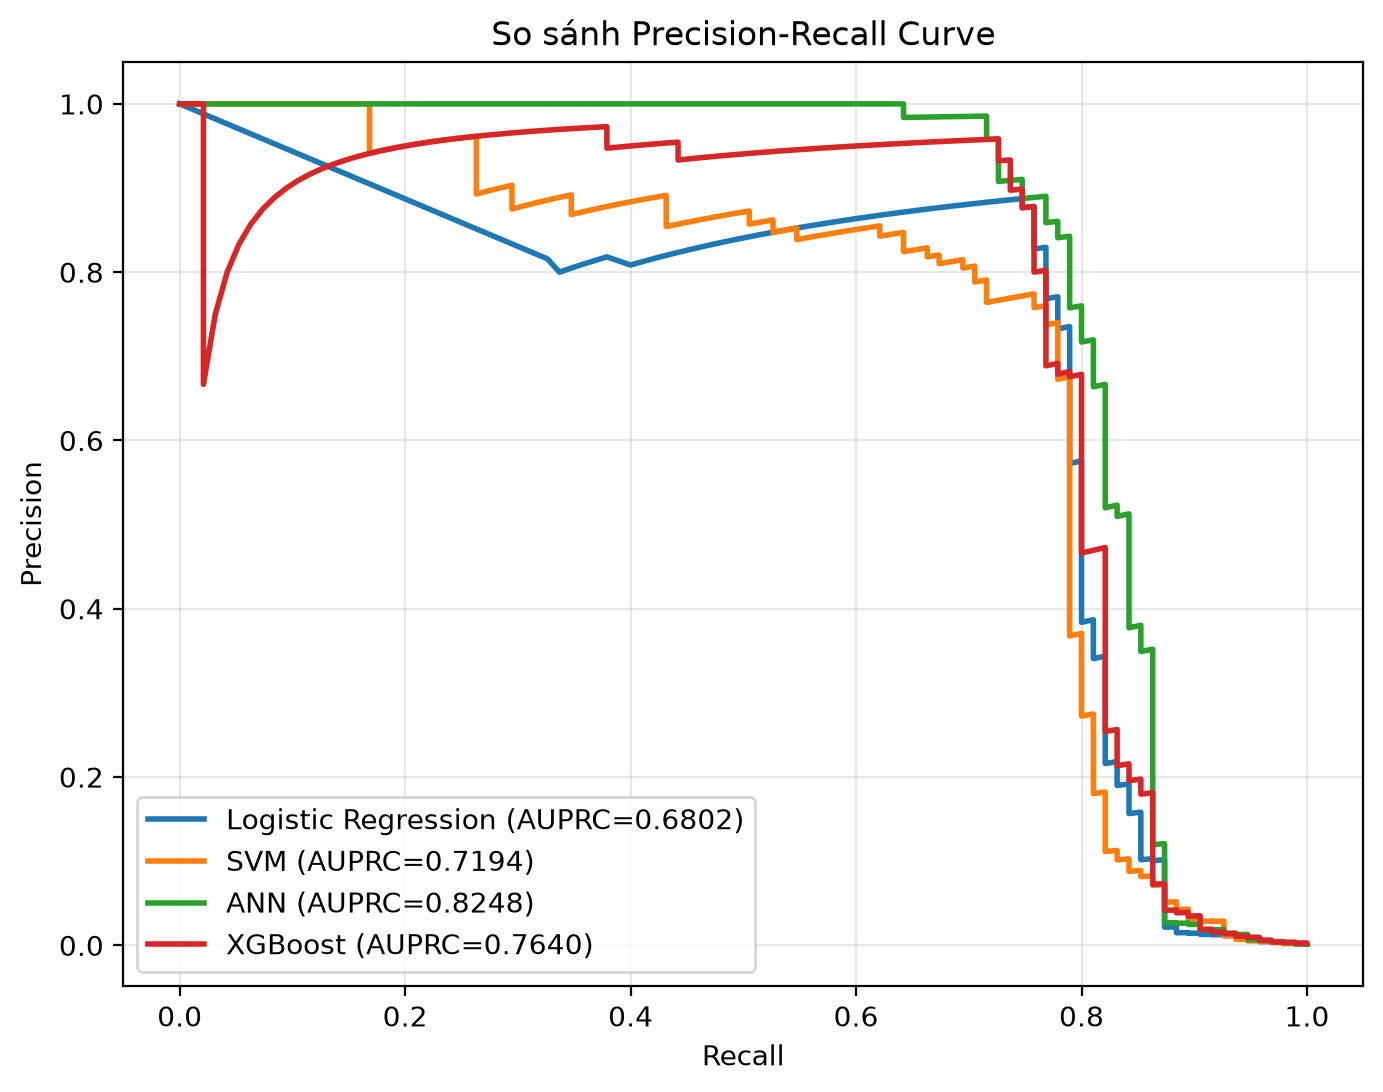
\includegraphics[width=0.8\linewidth]{graphics/compare_pr_curves.png}
\caption{So sánh đường cong Precision--Recall của các mô hình.}
\label{fig:so-sanh-pr}
\end{figure}

Hình~\ref{fig:so-sanh-metric} so sánh bốn metric chính giữa các mô hình. Có thể thấy Logistic Regression nổi bật ở Recall nhưng rất thấp ở Precision và F1, trong khi ANN và XGBoost cân bằng hơn giữa các metric.

\begin{figure}[H]
\centering
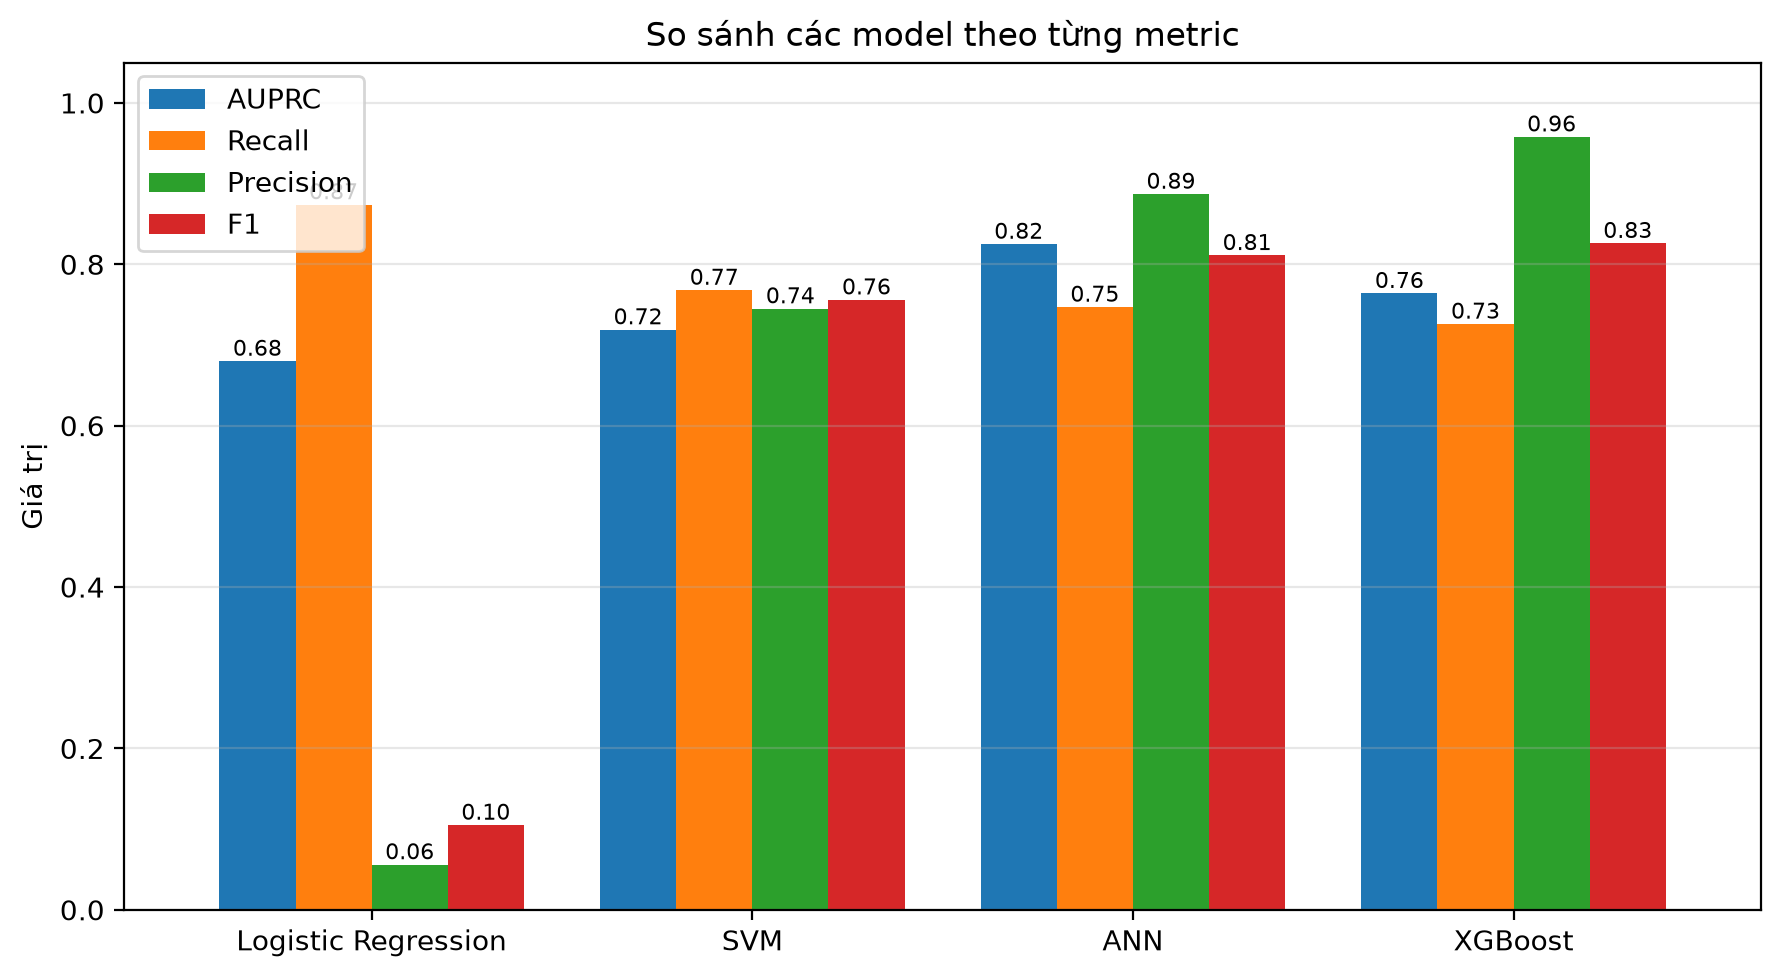
\includegraphics[width=0.85\linewidth]{graphics/compare_metrics_bar.png}
\caption{So sánh AUPRC, Recall, Precision và F1 của các mô hình.}
\label{fig:so-sanh-metric}
\end{figure}

Hình~\ref{fig:so-sanh-cm} thể hiện ma trận nhầm lẫn của từng mô hình tại $\tau = 0{,}5$ (hàng là nhãn dự đoán, cột là nhãn thực). Hình~\ref{fig:so-sanh-loi} cho thấy số lượng hai loại lỗi: $FN$ (bỏ sót gian lận) và $FP$ (báo nhầm giao dịch hợp lệ). Logistic Regression có ít $FN$ nhất ($12$) nhưng nhiều $FP$ nhất ($1\,403$), còn XGBoost có ít $FP$ nhất ($3$) nhưng nhiều $FN$ nhất ($26$).

\begin{figure}[H]
\centering
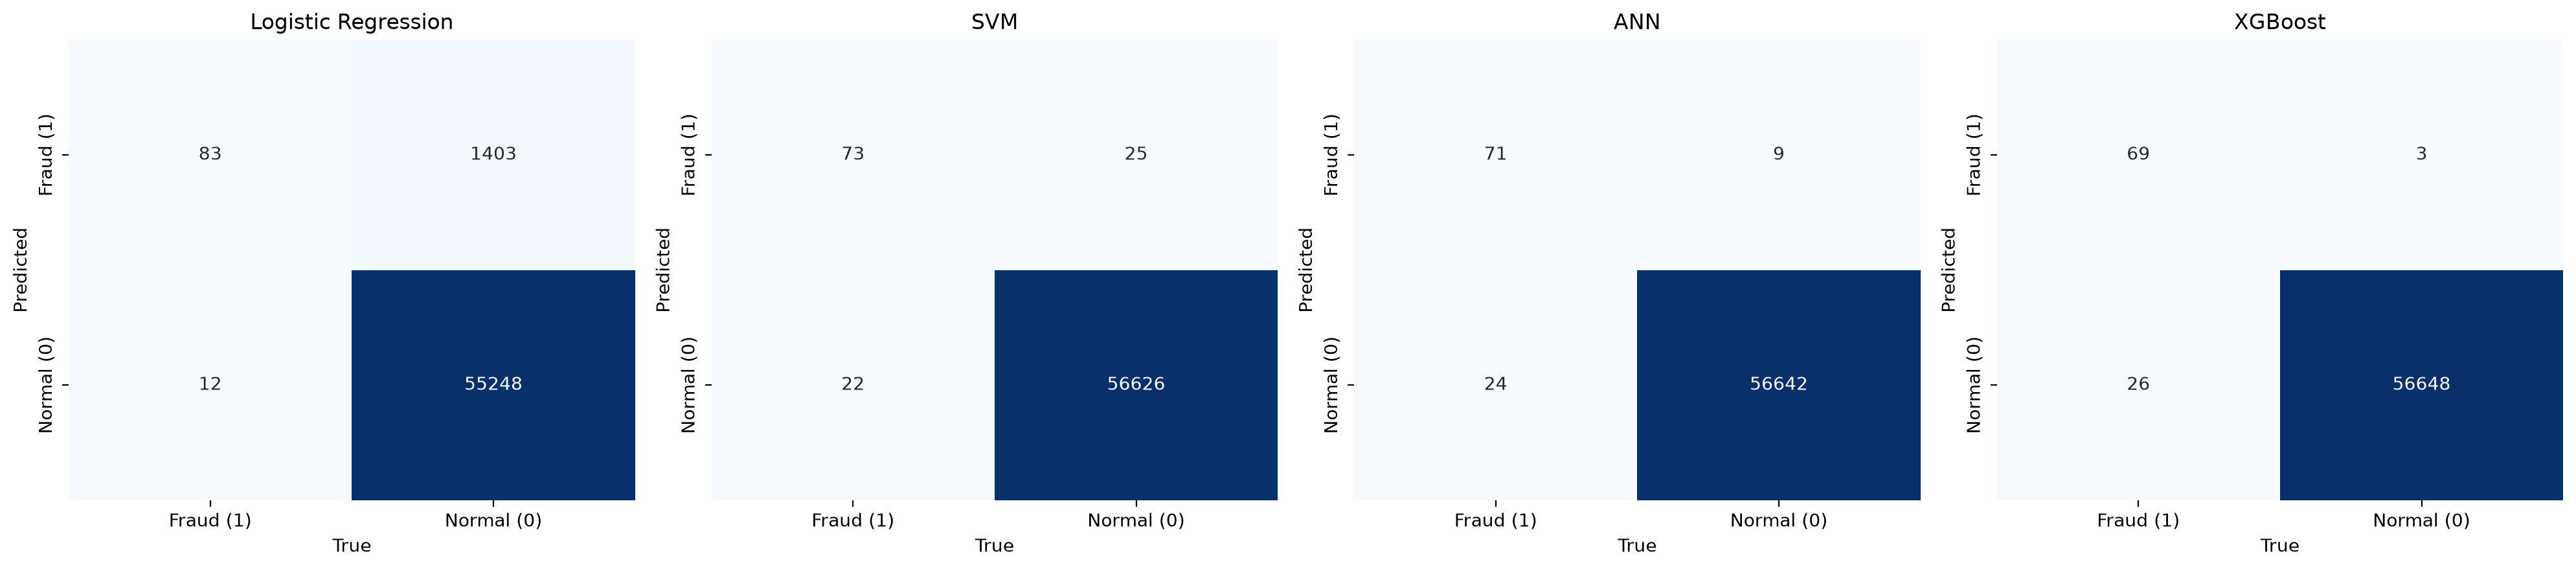
\includegraphics[width=\linewidth]{graphics/compare_confusion_matrices.png}
\caption{Ma trận nhầm lẫn của các mô hình trên tập kiểm tra ($\tau = 0{,}5$).}
\label{fig:so-sanh-cm}
\end{figure}

\begin{figure}[H]
\centering
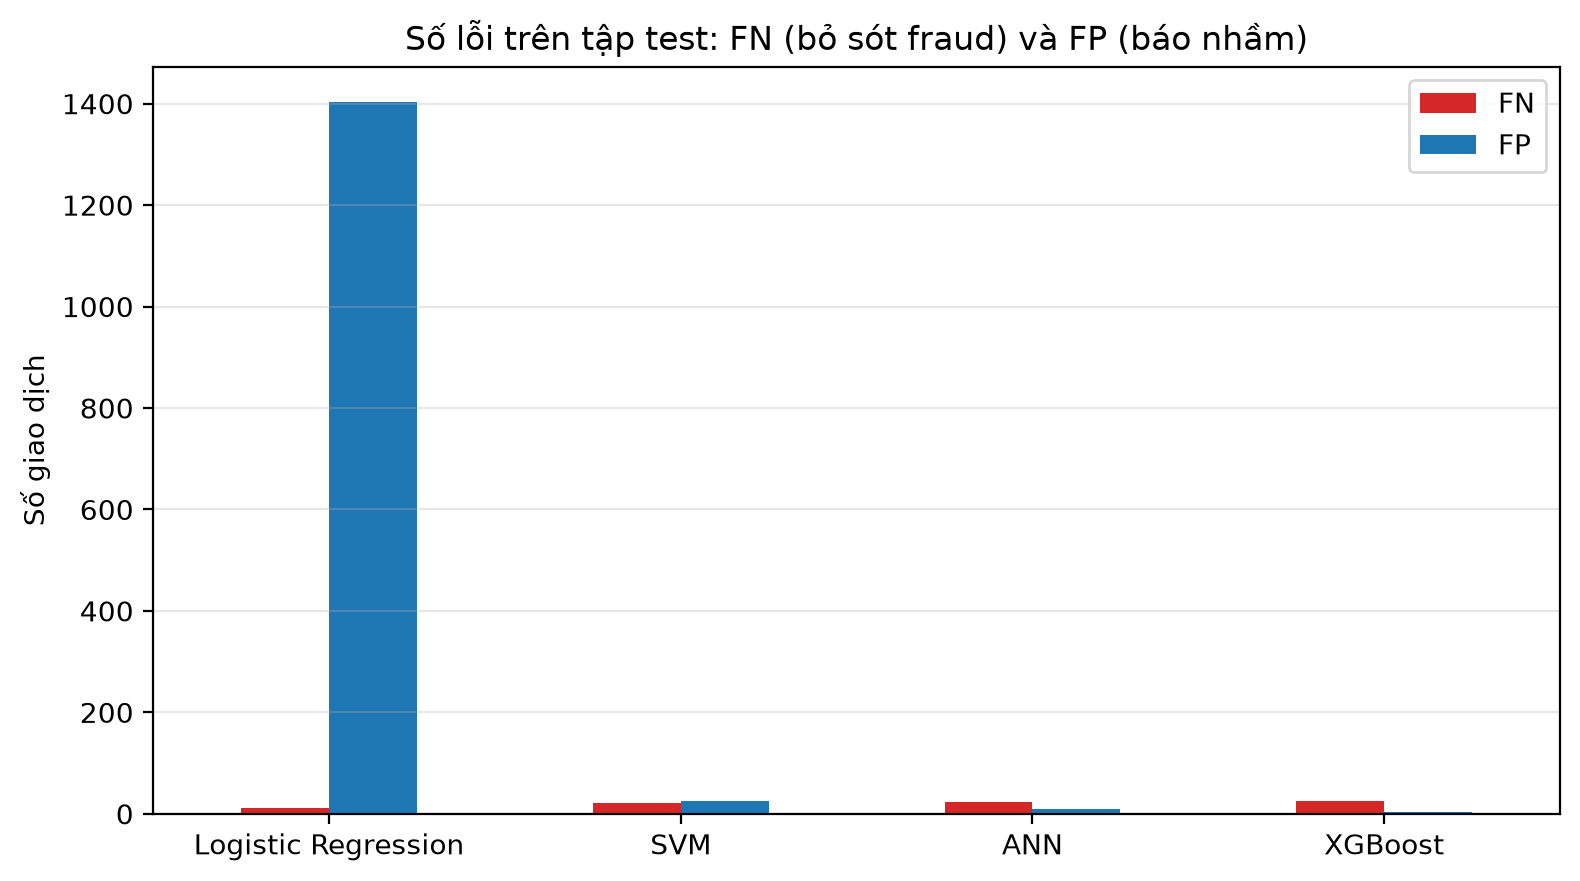
\includegraphics[width=0.75\linewidth]{graphics/compare_errors.png}
\caption{Số lượng $FN$ và $FP$ của các mô hình trên tập kiểm tra.}
\label{fig:so-sanh-loi}
\end{figure}

Cuối cùng, Hình~\ref{fig:threshold-sweep} thể hiện sự thay đổi của Precision, Recall và F1 theo ngưỡng $\tau$ cho từng mô hình. Với ANN và XGBoost, F1 duy trì ở mức khoảng $0{,}81$--$0{,}83$ trên một dải ngưỡng rộng (xấp xỉ $0{,}2$ đến $0{,}8$), nên ngưỡng mặc định $\tau = 0{,}5$ nằm trong vùng gần tối ưu và kết quả ít nhạy với ngưỡng. SVM cũng cho F1 ổn định ở mức $0{,}73$--$0{,}76$ khi $\tau \gtrsim 0{,}4$, nhưng F1 giảm mạnh khi $\tau$ nhỏ hơn khoảng $0{,}35$. Logistic Regression khác biệt rõ rệt: do dùng \texttt{class\_weight=balanced}, xác suất đầu ra bị đẩy cao nên Precision thấp hơn $0{,}2$ với mọi $\tau$ dưới khoảng $0{,}8$, và F1 chỉ tăng khi $\tau$ tiến gần $1$ (xấp xỉ $0{,}7$ tại $\tau \approx 0{,}99$). Như vậy, ngưỡng $0{,}5$ rất xa ngưỡng tối ưu của mô hình này, và F1 thấp ($0{,}105$) ở Bảng~\ref{tab:ket-qua-test} phần lớn là do ngưỡng chứ không hẳn do khả năng xếp hạng kém. Cần lưu ý rằng Hình~\ref{fig:threshold-sweep} được vẽ trên tập kiểm tra chỉ nhằm mục đích phân tích độ nhạy của các metric theo ngưỡng, các kết quả chính trong Bảng~\ref{tab:ket-qua-test} đều dùng ngưỡng cố định $\tau = 0{,}5$, không được điều chỉnh trên tập kiểm tra. Trong ứng dụng thực tế, ngưỡng cần được chọn trên tập validation hoặc bằng kiểm định chéo để tránh rò rỉ thông tin từ tập kiểm tra.

\begin{figure}[H]
\centering
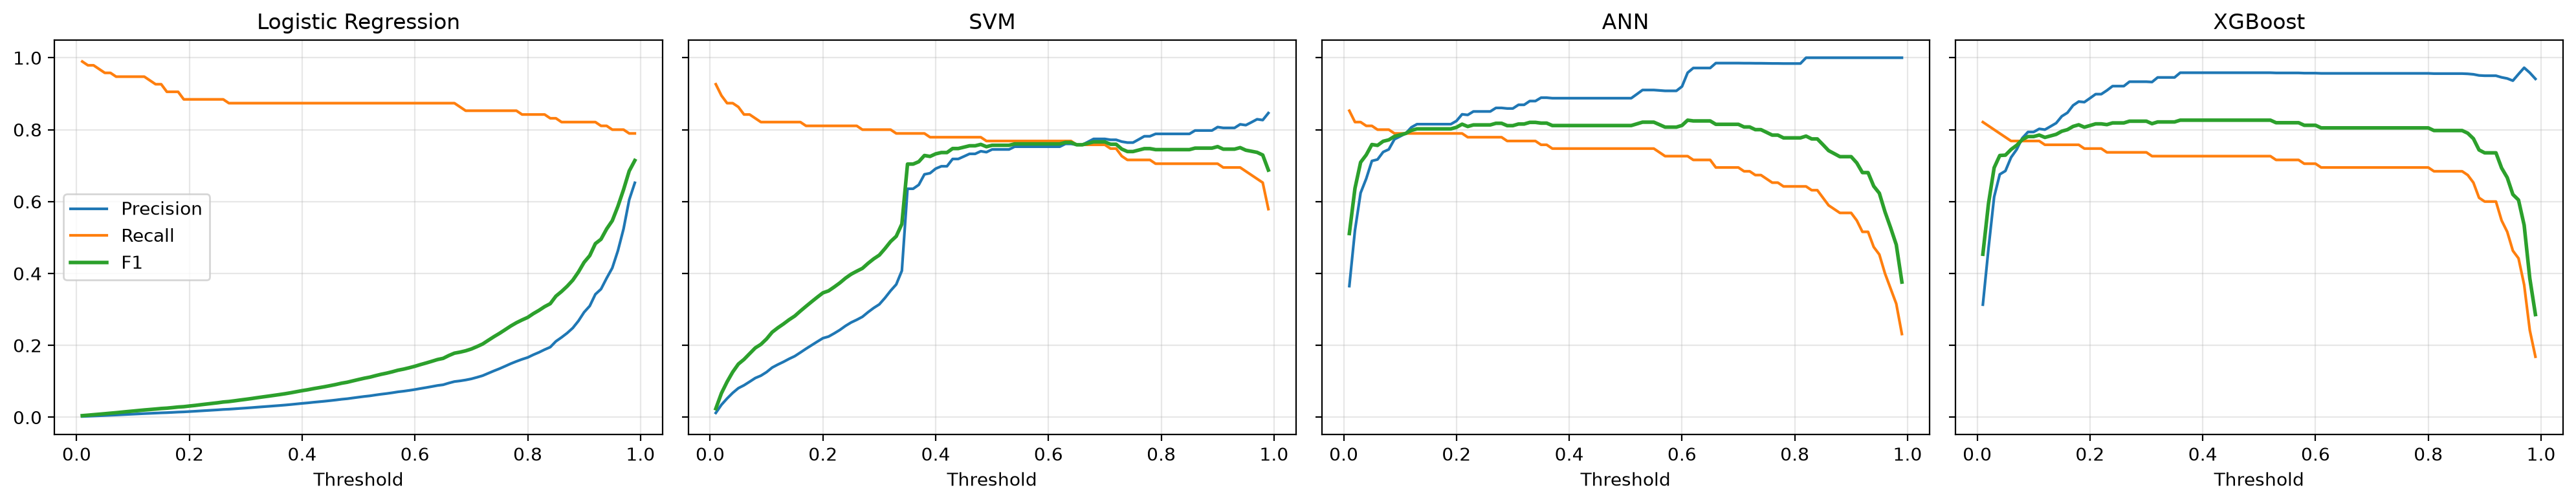
\includegraphics[width=\linewidth]{graphics/compare_threshold_sweep.png}
\caption{Precision, Recall và F1 theo ngưỡng quyết định $\tau$.}
\label{fig:threshold-sweep}
\end{figure}


% ==============================================================================
% 5. Thảo luận 
% ==============================================================================
\clearpage
\section{Thảo luận}\label{sec:thao-luan}
\subsection{Phân tích và so sánh giữa các mô hình}\label{subsec:phan-tich-so-sanh}

\subsubsection{Phân tích kết quả từng mô hình}

\paragraph{1. Logistic Regression (\texttt{src/model\_logistic.py})}\mbox{}
\begin{itemize}
    \item \textbf{Hiệu năng qua 5-fold CV:} Tại ngưỡng $t = 0.5$, mô hình đạt \texttt{AUPRC} ổn định trong khoảng $0.697 - 0.759$ (trung bình $\approx 0.740$) và \texttt{Recall} rất cao ($0.855 - 0.961$). Tuy nhiên, \texttt{Precision} chỉ dao động $0.049 - 0.064$ và \texttt{F1} đạt $0.093 - 0.119$.
    \item \textbf{Hiệu năng trên tập Test:} Mô hình đạt \texttt{AUPRC} $= 0.680$, \texttt{Recall} $= 0.874$ (phát hiện $83/95$ giao dịch gian lận, bỏ sót $\text{FN} = 12$), \texttt{Precision} $= 0.056$ ($\text{FP} = 1{,}403$ trên $56{,}651$ giao dịch bình thường) và \texttt{F1} $= 0.105$.
    \item \textbf{Ưu điểm:} Tốc độ huấn luyện nhanh, kiến trúc đơn giản dễ diễn giải trọng số và nhạy với lớp thiểu số (\texttt{Recall} cao), đóng vai trò mô hình cơ sở (\textit{baseline}) hiệu quả để sàng lọc gian lận.
    \item \textbf{Nhược điểm:} Do là bộ phân lớp tuyến tính nên không biểu diễn được các ranh giới phi tuyến phức tạp; đồng thời việc dùng \texttt{class\_weight="balanced"} khiến mô hình tạo nhiều cảnh báo giả tại ngưỡng mặc định $t = 0.5$.
\end{itemize}

\paragraph{2. Support Vector Machine -- Kernel RBF (\texttt{src/model\_svm.py})}\mbox{}
\begin{itemize}
    \item \textbf{Hiệu năng qua 5-fold CV:} Mô hình đạt \texttt{AUPRC} từ $0.672$ đến $0.807$ (Fold 4 cao nhất đạt $0.807$), \texttt{Recall} trong khoảng $0.737 - 0.868$, \texttt{Precision} đạt $0.492 - 0.735$ và \texttt{F1} đạt $0.628 - 0.772$.
    \item \textbf{Hiệu năng trên tập Test:} Tại $t = 0.5$, mô hình đạt \texttt{AUPRC} $= 0.719$, \texttt{Recall} $= 0.768$ ($73/95$ ca gian lận, $\text{FN} = 22$), \texttt{Precision} $= 0.745$ (chỉ $\text{FP} = 25$ ca báo nhầm) và \texttt{F1} $= 0.756$.
    \item \textbf{Ưu điểm:} Ranh giới phi tuyến của hạt nhân RBF kết hợp chuẩn hóa \texttt{StandardScaler} và giảm mẫu \texttt{RandomUnderSampler(0.05)} giúp cân bằng tốt \texttt{Precision}--\texttt{Recall} ngay tại $t = 0.5$, giảm hơn $56$ lần số cảnh báo giả so với Logistic Regression.
    \item \textbf{Nhược điểm:} Độ nhạy \texttt{Recall} tại $t = 0.5$ thấp hơn Logistic Regression (sót thêm $10$ ca gian lận), thời gian huấn luyện lâu hơn và kết quả giữa các \textit{fold} biến thiên nhẹ do lấy mẫu ngẫu nhiên lớp đa số.
\end{itemize}

\paragraph{3. Artificial Neural Network -- ANN (\texttt{src/model\_ANN.py})}\mbox{}
\begin{itemize}
    \item \textbf{Hiệu năng qua 5-fold CV:} Tại ngưỡng $t = 0.5$, mô hình đạt \texttt{AUPRC} cao trong khoảng $0.723 - 0.870$ (trung bình $\approx 0.818$, cao nhất ở Fold 5 đạt $0.870$), \texttt{Recall} dao động $0.653 - 0.882$, \texttt{Precision} rất cao từ $0.788$ đến $1.000$ (Fold 1 không có báo nhầm nào, $\text{FP} = 0$) và \texttt{F1} đạt $0.741 - 0.855$.
    \item \textbf{Hiệu năng trên tập Test:} Mô hình đạt \texttt{AUPRC} $= 0.825$ (cao nhất trong 4 mô hình), \texttt{Recall} $= 0.747$ (phát hiện $71/95$ ca gian lận, bỏ sót $\text{FN} = 24$), \texttt{Precision} $= 0.887$ (chỉ $\text{FP} = 9$ ca báo nhầm trên $56{,}651$ giao dịch bình thường, $\text{TN} = 56{,}642$) và \texttt{F1} $= 0.811$.
    \item \textbf{Ưu điểm:} Kiến trúc mạng hai tầng ẩn \texttt{(64, 32)} kết hợp hàm kích hoạt ReLU và cơ chế \texttt{early\_stopping=True} giúp học tốt các đặc trưng phi tuyến phức tạp, đạt năng lực xếp hạng xác suất tổng thể (\texttt{AUPRC}) cao nhất đồng thời duy trì tỷ lệ báo nhầm rất thấp ngay tại ngưỡng mặc định $t = 0.5$.
    \item \textbf{Nhược điểm:} Do huấn luyện trên phân phối gốc mất cân bằng mà không áp dụng trọng số lớp nên độ nhạy \texttt{Recall} tại $t = 0.5$ còn bảo thủ (bỏ sót $24$ ca gian lận); hiệu năng giữa các \textit{fold} có độ dao động nhất định (Fold 3 giảm xuống \texttt{AUPRC} $= 0.723$), ít khả năng diễn giải trực tiếp như mô hình tuyến tính và nhạy với siêu tham số khởi tạo.
\end{itemize}

\paragraph{4. Ensemble Learning -- XGBoost (\texttt{src/model\_ensemble.py})}\mbox{}
\begin{itemize}
    \item \textbf{Hiệu năng qua 5-fold CV:} Mô hình duy trì độ ổn định rất cao qua 5 \textit{folds} với \texttt{AUPRC} từ $0.782$ đến $0.859$ (trung bình $\approx 0.822$, cao nhất ở Fold 5 đạt $0.859$), \texttt{Recall} trong khoảng $0.680 - 0.816$, \texttt{Precision} luôn ở mức rất cao ($0.886 - 0.983$) và \texttt{F1} đạt $0.779 - 0.874$.
    \item \textbf{Hiệu năng trên tập Test:} Tại $t = 0.5$, mô hình đạt \texttt{AUPRC} $= 0.764$, \texttt{Recall} $= 0.726$ ($69/95$ ca gian lận, $\text{FN} = 26$), \texttt{Precision} $= 0.958$ (chỉ $\text{FP} = 3$ ca báo nhầm trên $56{,}651$ giao dịch bình thường, $\text{TN} = 56{,}648$) và \texttt{F1} $= 0.826$ (cao nhất trong 4 mô hình tại $t = 0.5$).
    \item \textbf{Ưu điểm:} Tổ hợp 100 cây quyết định nông (\texttt{max\_depth=3}) kết hợp điều chuẩn L2 và thuật toán \texttt{tree\_method="hist"} cho tốc độ huấn luyện rất nhanh, ít biến thiên giữa các \textit{fold} và gần như triệt tiêu cảnh báo giả ($\text{FP} = 3$, \texttt{Precision} $= 95.8\%$), rất phù hợp với dữ liệu bảng.
    \item \textbf{Nhược điểm:} Do chưa thiết lập trọng số lớp (\texttt{scale\_pos\_weight}) hoặc hạ ngưỡng quyết định nên mô hình có xu hướng thận trọng với lớp thiểu số, dẫn đến \texttt{Recall} trên tập Test ($0.726$) thấp nhất trong 4 mô hình tại $t = 0.5$ và \texttt{AUPRC} trên Test ($0.764$) có độ sụt giảm nhẹ so với trung bình CV ($0.822$).
\end{itemize}

\subsubsection{Phân tích so sánh các mô hình tại ngưỡng $t = 0.5$}

Bảng~\ref{tab:compare_4_models_t05} tổng hợp kết quả đánh giá của bốn mô hình trên tập Test tại ngưỡng mặc định $t = 0.5$ sử dụng bộ độ đo thống nhất từ \texttt{src/metrics.py}.

\begin{table}[H]
\centering
\caption{So sánh hiệu năng 4 mô hình trên tập Test tại ngưỡng $t = 0.5$ (\texttt{src/metrics.py})}
\label{tab:compare_4_models_t05}
\renewcommand{\arraystretch}{1.2}
\begin{tabular}{|l|c|c|c|c|c|c|c|c|}
\hline
\textbf{Mô hình} & \textbf{AUPRC} & \textbf{Recall} & \textbf{Precision} & \textbf{F1} & \textbf{TP} & \textbf{FP} & \textbf{FN} & \textbf{TN} \\
\hline
Logistic Regression & $0.680$ & $\mathbf{0.874}$ & $0.056$ & $0.105$ & $83$ & $1403$ & $12$ & $55248$ \\
\hline
SVM (RBF) & $0.719$ & $0.768$ & $0.745$ & $0.756$ & $73$ & $25$ & $22$ & $56626$ \\
\hline
ANN & $\mathbf{0.825}$ & $0.747$ & $0.887$ & $0.811$ & $71$ & $9$ & $24$ & $56642$ \\
\hline
XGBoost & $0.764$ & $0.726$ & $\mathbf{0.958}$ & $\mathbf{0.826}$ & $69$ & $3$ & $26$ & $56648$ \\
\hline
\end{tabular}
\end{table}

\begin{itemize}
    \item \textbf{Chỉ số \texttt{AUPRC}:} \textbf{ANN} dẫn đầu toàn diện với \texttt{AUPRC} $= 0.825$, theo sau là \textbf{XGBoost} ($0.764$), đều vượt trội rõ rệt so với hai mô hình baseline là SVM ($0.719$) và Logistic Regression ($0.680$). Kết quả này cho thấy khả năng học biểu diễn phi tuyến nhiều tầng của ANN giúp tách biệt và xếp hạng xác suất giữa giao dịch gian lận và bình thường hiệu quả nhất trên toàn bộ dải ngưỡng.
    \item \textbf{Chỉ số \texttt{Recall}:} Ở ngưỡng $t = 0.5$, \textbf{Logistic Regression} đạt độ nhạy cao nhất ($0.874$, bắt được $83/95$ ca) nhờ \texttt{class\_weight="balanced"} phạt nặng lỗi bỏ sót ($\sim 600$ lần), tiếp đến là SVM ($0.768$, $73/95$), ANN ($0.747$, $71/95$) và thấp nhất là XGBoost ($0.726$, $69/95$). Nguyên nhân ANN và XGBoost có \texttt{Recall} bảo thủ hơn tại $t = 0.5$ là vì cả hai được huấn luyện trực tiếp trên phân phối dữ liệu gốc mất cân bằng cực mạnh mà chưa điều chỉnh trọng số lớp hay hạ ngưỡng quyết định.
    \item \textbf{Chỉ số \texttt{Precision}:} \textbf{XGBoost} vượt trội tuyệt đối với \texttt{Precision} $= 0.958$ (chỉ $3$ ca báo nhầm trên $56{,}651$ giao dịch bình thường), đứng thứ hai là \textbf{ANN} ($0.887$, $\text{FP} = 9$), bỏ xa SVM ($0.745$, $\text{FP} = 25$) và Logistic Regression ($0.056$, $\text{FP} = 1{,}403$). Nhờ giữ nguyên phân phối gốc cùng cơ chế điều chuẩn cây nông và dừng sớm, cả XGBoost lẫn ANN đều hạn chế tối đa cảnh báo giả.
    \item \textbf{Chỉ số \texttt{F1}:} Vì \texttt{F1} là trung bình điều hòa giữa \texttt{Precision} và \texttt{Recall}, \textbf{XGBoost} đạt mức cân bằng cao nhất tại ngưỡng mặc định $t = 0.5$ với \texttt{F1} $= 0.826$, nhỉnh hơn \textbf{ANN} ($0.811$) và vượt xa SVM ($0.756$) cũng như Logistic Regression ($0.105$). Xét tổng thể tại $t = 0.5$, XGBoost phù hợp nhất cho yêu cầu chính xác cao và ít làm phiền khách hàng, trong khi ANN sở hữu tiềm năng xếp hạng xác suất (\texttt{AUPRC}) tốt nhất nếu tiếp tục tinh chỉnh ngưỡng quyết định để đẩy cao \texttt{Recall}.
\end{itemize}

\subsubsection{Phân tích Precision thấp của Logistic Regression và tác động khi điều chỉnh ngưỡng $t$}

Tại ngưỡng mặc định $t = 0.5$, \texttt{Precision} của Logistic Regression chỉ đạt $0.056$ ($5.6\%$, tức rất thấp dù \texttt{AUPRC} $= 0.680$ vẫn tốt). Nguyên nhân đến từ hai yếu tố cộng hưởng: (1) \textbf{mất cân bằng nền cực đoan} ($56{,}651$ mẫu bình thường so với $95$ mẫu gian lận trên tập Test) khiến chỉ $2.48\%$ tỷ lệ báo nhầm trên lớp \texttt{Normal} cũng tạo ra tới $\text{FP} = 1{,}403$; và (2) tham số \texttt{class\_weight="balanced"} làm dịch xác suất dự đoán $\hat{p}$ lên rất cao, khiến mốc $t = 0.5$ trở thành ngưỡng cắt quá thấp.

Bảng~\ref{tab:lr_threshold_sweep} trình bày kết quả thực nghiệm khi giữ nguyên mô hình Logistic Regression đã huấn luyện và tăng dần ngưỡng quyết định $t$:

\begin{table}[H]
\centering
\caption{Biến thiên các chỉ số của Logistic Regression trên tập Test khi tăng ngưỡng $t$}
\label{tab:lr_threshold_sweep}
\renewcommand{\arraystretch}{1.2}
\begin{tabular}{|c|c|c|c|c|c|c|c|}
\hline
\textbf{Ngưỡng $t$} & \textbf{AUPRC} & \textbf{Precision} & \textbf{Recall} & \textbf{F1} & \textbf{TP} & \textbf{FP} & \textbf{FN} \\
\hline
$0.500000$ (mặc định) & $0.680$ & $0.056$ & $\mathbf{0.874}$ & $0.105$ & $83$ & $1403$ & $12$ \\
\hline
$0.900000$ & $0.680$ & $0.292$ & $0.821$ & $0.431$ & $78$ & $189$ & $17$ \\
\hline
$0.990000$ & $0.680$ & $0.652$ & $0.789$ & $0.714$ & $75$ & $40$ & $20$ \\
\hline
$0.999000$ & $0.680$ & $0.771$ & $0.779$ & $0.775$ & $74$ & $22$ & $21$ \\
\hline
$0.999900$ & $0.680$ & $0.793$ & $0.768$ & $0.781$ & $73$ & $19$ & $22$ \\
\hline
$0.999999$ (tối ưu OOF) & $0.680$ & $\mathbf{0.878}$ & $0.758$ & $\mathbf{0.814}$ & $72$ & $\mathbf{10}$ & $23$ \\
\hline
\end{tabular}
\end{table}

Từ Bảng~\ref{tab:lr_threshold_sweep}, việc điều chỉnh tăng ngưỡng $t$ mang lại ba ý nghĩa quan trọng:
\begin{enumerate}
    \item \textbf{Khẳng định năng lực thực chất của mô hình:} Chỉ số \texttt{AUPRC} $= 0.680$ giữ nguyên không đổi theo $t$. Khi nâng ngưỡng lên $t = 0.999$ hoặc ngưỡng tối ưu $t = 0.999999$ (xác định qua kiểm định chéo \textit{Out-Of-Fold}), \texttt{Precision} tăng mạnh từ $5.6\%$ lên $77.1\% - 87.8\%$, số cảnh báo giả giảm hơn $140$ lần (từ $1{,}403$ xuống còn $10$ ca), đưa \texttt{F1} lên tới $0.814$. Điều này chứng minh nhược điểm tại $t = 0.5$ hoàn toàn nằm ở điểm cắt xác suất chứ không phải do mô hình học kém.
    \item \textbf{Làm rõ sự đánh đổi Precision--Recall:} Khi tăng $t$ từ $0.5$ lên $0.999999$, \texttt{Precision} tăng vọt nhưng \texttt{Recall} giảm tương ứng từ $0.874$ xuống $0.758$ (bỏ sót thêm $11$ ca gian lận). Ngược lại, từ mốc $0.999999$ hạ xuống $0.5$, để bắt thêm $11$ ca gian lận phải đánh đổi bằng $1{,}393$ ca báo nhầm thêm.
    \item \textbf{Ý nghĩa triển khai thực tế:} Khi áp dụng \texttt{class\_weight="balanced"}, cần tinh chỉnh ngưỡng $t$ trên tập kiểm định chéo thay vì dùng cứng $t = 0.5$. Tùy mục tiêu nghiệp vụ ngân hàng, hệ thống có thể chọn $t \approx 0.999999$ nếu muốn tự động khóa thẻ chính xác cao, hoặc chọn ngưỡng trung gian ($t \approx 0.99$) để yêu cầu xác thực bổ sung (OTP) nhằm vừa giữ \texttt{Recall} cao vừa tránh quá tải cảnh báo giả.
\end{enumerate}

% Phụ trách: Hiền
% Nhiệm vụ báo cáo: Thảo luận — Hạn chế và thách thức

\subsection{Hạn chế và thách thức}\label{subsec:han-che-thach-thuc}
% TODO (Hiền):
% - Các hạn chế của dữ liệu (đặc trưng PCA ẩn danh, mất cân bằng lớp, thiếu thông tin ngữ cảnh...).
% - Hạn chế của phương pháp thử nghiệm (thời gian huấn luyện, độ nhạy với ngưỡng phân loại, khả năng tổng quát hóa...).

\textit{[Nội dung mục Hạn chế và thách thức đang chờ hoàn thiện.]}


% ==============================================================================
% 6. Kết luận và hướng phát triển
% ==============================================================================
\clearpage
\section{Kết luận và hướng phát triển}\label{sec:ket-luan}
% Phụ trách: Hiền
% Nhiệm vụ báo cáo: Kết luận và hướng phát triển — Kết luận

\subsection{Kết luận}\label{subsec:ket-luan}
% TODO (Hiền):
% - Tóm tắt lại toàn bộ quy trình đã thực hiện (tiền xử lý, xây dựng baseline, mô hình nâng cao, đánh giá).
% - Nhấn mạnh những kết quả chính đạt được và mô hình tốt nhất cho bài toán.

\textit{[Nội dung mục Kết luận đang chờ hoàn thiện.]}

% Phụ trách: Hiền
% Nhiệm vụ báo cáo: Kết luận và hướng phát triển — Hướng phát triển

\subsection{Hướng phát triển}\label{subsec:huong-phat-trien}
% TODO (Hiền):
% - Đề xuất các hướng cải tiến trong tương lai (tối ưu siêu tham số sâu hơn, cân bằng dữ liệu nâng cao, học sâu / anomaly detection, triển khai thành dịch vụ real-time...).

\textit{[Nội dung mục Hướng phát triển đang chờ hoàn thiện.]}


% ==============================================================================
% Tài liệu tham khảo
% ==============================================================================
\clearpage
\bibliographystyle{plain}
\bibliography{refs/example.bib}
\nocite{*}

\end{document}
